\documentclass{article}

% Recommended packages for ICML
\usepackage{microtype}
\usepackage{graphicx}
\usepackage{booktabs}

\usepackage{algorithm}
\usepackage{algorithmic}
\providecommand{\theHalgorithm}{\arabic{algorithm}}

\usepackage[hyperfootnotes=false]{hyperref}
\hypersetup{hidelinks}

% Use the ICML layout while providing the thesis title-page information
% separately and suppressing the conference-style notice.
\usepackage[preprint]{icml2026}
\hypersetup{
  pdftitle={Operational Boundaries of a Modular Recurrent-Memory Architecture in Partially Observable Reinforcement Learning},
  pdfauthor={Tim Schweitzer},
  pdfsubject={Master's thesis manuscript},
  pdfkeywords={partially observable reinforcement learning, recurrent memory, associative memory}
}

% Math packages
\usepackage{amsmath}
\usepackage{amssymb}
\usepackage{mathtools}
\usepackage{amsthm}
\usepackage{listings}
\usepackage{xcolor}
\usepackage{tabularx}
\usepackage{tikz}
\usetikzlibrary{shapes.geometric, arrows, positioning}

\usepackage{placeins}
\usepackage{balance}
\usepackage{float}
\newcolumntype{Y}{>{\centering\arraybackslash}X}

% Cleveref for formatting cross-references
\usepackage[capitalize,noabbrev]{cleveref}

% Listing styling for code blocks
\definecolor{codegreen}{rgb}{0,0.6,0}
\definecolor{codegray}{rgb}{0.5,0.5,0.5}
\definecolor{codepurple}{rgb}{0.58,0,0.82}
\definecolor{backcolour}{rgb}{0.96,0.96,0.96}
\definecolor{thesisblue}{RGB}{31,78,121}

\lstdefinestyle{mystyle}{
    backgroundcolor=\color{backcolour},   
    commentstyle=\color{codegreen},
    keywordstyle=\color{magenta},
    numberstyle=\tiny\color{codegray},
    stringstyle=\color{codepurple},
    basicstyle=\ttfamily\scriptsize,
    breakatwhitespace=false,         
    breaklines=true,                 
    captionpos=b,                    
    keepspaces=true,                 
    numbers=left,                    
    numbersep=5pt,                  
    showspaces=false,                
    showstringspaces=false,
    showtabs=false,                  
    tabsize=2
}
\lstset{style=mystyle}

% Theorems
\theoremstyle{plain}
\newtheorem{theorem}{Theorem}[section]
\newtheorem{proposition}[theorem]{Proposition}
\newtheorem{lemma}[theorem]{Lemma}
\newtheorem{corollary}[theorem]{Corollary}
\theoremstyle{definition}
\newtheorem{definition}[theorem]{Definition}
\newtheorem{assumption}[theorem]{Assumption}
\theoremstyle{remark}
\newtheorem{remark}[theorem]{Remark}

% Running title
\icmltitlerunning{Operational Boundaries in Partially Observable RL}

\begin{document}

\pagenumbering{gobble}
\begin{titlepage}
\thispagestyle{empty}
\centering
\vspace*{1.3cm}
{\large Ravensburg-Weingarten University of Applied Sciences (RWU)\par}

\vspace{1.7cm}
{\color{thesisblue}\rule{0.72\textwidth}{1.1pt}\par}
\vspace{1.25cm}
{\Large\bfseries Master's Thesis\par}
\vspace{1.05cm}
{\LARGE\bfseries
Operational Boundaries of a Modular Recurrent-Memory Architecture in Partially Observable Reinforcement Learning\par}
\vspace{1.25cm}
{\color{thesisblue}\rule{0.72\textwidth}{1.1pt}\par}

\vfill
{\large Tim Schweitzer\par}
\vspace{0.25cm}
{\normalsize Matrikelnummer: 29844429\par}
\vspace{0.45cm}
{\normalsize October 2026\par}
\vspace*{1.3cm}
\end{titlepage}

\clearpage
\pagenumbering{arabic}

\twocolumn[
\icmltitle{Operational Boundaries of a Modular Recurrent-Memory Architecture in Partially Observable Reinforcement Learning}

\begin{center}
\textbf{Tim Schweitzer}
\end{center}

\begin{abstract}
Partially observable reinforcement learning requires retention, associative retrieval, and revision under computational constraints, but whole-model rankings obscure these distinct demands. We introduce Stabilized decoupled Linear Gated Recurrence (SdLG), a modular architecture with configurable associative execution, positional phase, local processing, and gradient routing. Evaluations across Passive T-Maze, DoorKey, POPGym, and Craftax reveal task- and configuration-dependent architecture rankings. On Passive T-Maze, GTrXL-128 reaches mean return $1.000$ at the trained horizon but falls to $0.503$ at the unseen horizon $H=200$, whereas SdLG-Exact changes from $0.900$ to $0.851$. Exact also achieves the highest observed mean return and success rate in the five-seed DoorKey comparison with GRU and GTrXL. Synthetic diagnostics show greater sensitivity to addressing than value dimension and a replacement--preservation trade-off. Factorization reduces carried-state memory without reducing batch-256 latency. Together, the results characterize the tested operating boundaries rather than establishing a universally superior architecture.
\end{abstract}
]

% The thesis title page carries the institutional and author information.
\makeatletter
\global\icml@noticeprintedtrue
\makeatother

\section{Introduction}
\label{sec:intro}

Recurrent memory in partially observable reinforcement learning must do more than retain a distant observation: an agent may need to address an association, revise it without damaging others, and execute the resulting state efficiently. Overall return conflates these demands. Online learning adds another distinction because recurrent state can cross truncated backpropagation through time (TBPTT) boundaries even when gradients cannot; forward retention is therefore not long-range credit assignment.

We develop Stabilized decoupled Linear Gated Recurrence (SdLG), a recurrent PPO architecture with gated associative memory, configurable execution, positional phase, local processing, and actor-gradient routing. We evaluate its configurations against established recurrent baselines, including GRU, LSTM, Mamba, GLA, and GTrXL, across complementary delayed-retention, spatial-control, POPGym, and Craftax protocols. Formulation controls and independent synthetic diagnostics then examine specific architectural choices and associative-memory operations.

Many of these mechanisms were developed for sequence modeling in language rather than online reinforcement learning. We ask whether they carry over to recurrent PPO in partially observable tasks: where do they help, where do they fail to help, and what do they cost?

Here, \emph{operational boundaries} are the tested tasks, memory operations, configurations, horizons, and execution costs under which a mechanism helps, fails to help, or introduces a trade-off. They are not a discovered maximum retention horizon or a universal performance frontier.

Our contributions are as follows:
\begin{enumerate}
    \item \textbf{Architecture integration:} a configurable recurrent PPO architecture combining associative execution, positional phase, local processing, and actor-gradient-routing mechanisms.
    \item \textbf{Memory behavior:} cross-task comparisons on T-Maze, DoorKey, and POPGym, plus independent retrieval and reassignment diagnostics.
    \item \textbf{Operational trade-offs:} configuration-specific component interventions and systems measurements distinguishing carried-state size, latency, and training-loop throughput.
\end{enumerate}

\section{Related Work}
\label{sec:related}

\paragraph{Recurrent memory in partially observable RL.}
Partially observable agents construct state from observation histories~\cite{kaelbling1998planning,sutton2018reinforcement}. LSTM and GRU are standard gated baselines~\cite{hochreiter1997long,cho2014learning}; GTrXL modifies Transformer-XL for stable RL training~\cite{parisotto2020stabilizing}. Recurrent agents are commonly used POMDP baselines~\cite{ni2022recurrent}, while recent studies distinguish memory from long-term credit assignment and compare recurrent and Transformer inductive biases~\cite{ni2023when,lu2024rethinking}.
Recent RL-specific work broadens this picture: memory traces provide compact exponential summaries with theoretical analysis and online-control experiments, while Memory Gym reports different GRU and Transformer-XL orderings across finite and endless memory tasks~\cite{eberhard2025memory,pleines2025memorygym}. Together, these studies motivate evaluating both memory representation and task regime.

\paragraph{Linear attention, state-space, and associative recurrence.}
Linear Transformers express kernel attention as recurrent outer-product state~\cite{katharopoulos2020transformers}, and fast-weight programmers make the key--value interpretation explicit~\cite{schlag2021linear}. GLA adds data-dependent gating~\cite{yang2024gated}; DeltaNet adds targeted Delta-rule correction~\cite{yang2024delta}; and Gated DeltaNet combines correction with forgetting gates and studies sliding-window hybrids~\cite{yang2025gateddelta}. SdLG-Exact instead uses the normalized gated additive recurrence defined in Section~\ref{sec:method}; the Delta rule is evaluated only in synthetic diagnostics. Other recurrent designs include RetNet, mLSTM, Mamba, and AGaLiTe's compact factorized recurrence~\cite{sun2023retentive,beck2024xlstm,gu2023mamba,pramanik2024agalite}. SdLG-Approx modifies the latter design for the evaluated online-RL configurations.

\par\vspace{0.45\baselineskip}\noindent\textbf{Local--global processing.}
Griffin interleaves recurrent and local-attention temporal-mixing blocks across depth~\cite{de2024griffin}. SdLG instead applies sliding-window attention and then associative recurrence sequentially inside each reference block. RoPE supplies the separately controlled positional phase~\cite{su2024roformer}.

\par\vspace{0.45\baselineskip}\noindent\textbf{Shared actor--critic representations.}
PPG separates policy/value optimization into phases, DAAC/IDAAC separates representations and adds invariance objectives, and PCGrad projects conflicting task gradients~\cite{cobbe2021phasic,raileanu2021decoupling,yu2020gradient}. These are distinct from SdLG's actor-gradient scaling during simultaneous actor--critic training.

\paragraph{Research gap and contribution.}
Prior work establishes gated associative recurrence, factorized recurrent state, local--global processing, and methods for managing actor--critic optimization across sequence modeling and online RL. Results obtained under different architectures, objectives, and tasks do not directly determine how these mechanisms behave when integrated into recurrent PPO across separate measurements of retention, retrieval, revision, and execution cost. SdLG does not claim invention of these individual mechanisms; its contribution is their implemented integration, configuration-specific adaptation, and empirical characterization through controlled diagnostics and task-level comparisons.

\section{SdLG Architecture and Controlled Modifications}
\label{sec:method}

SdLG-Exact is the reference recurrent-memory architecture. Sliding-window
attention (SWA) retains addressable recent features, and a normalized
full-matrix recurrence accumulates longer-range associations. Within every
reference block, SWA changes the representation before the associative stage
projects its queries, keys, and values. This differs from Griffin's
interleaving of recurrent and local-attention blocks across depth~\cite{de2024griffin};
SdLG has neither parallel local/global branches nor disjoint feature channels.

\begin{figure*}[t]
\centering
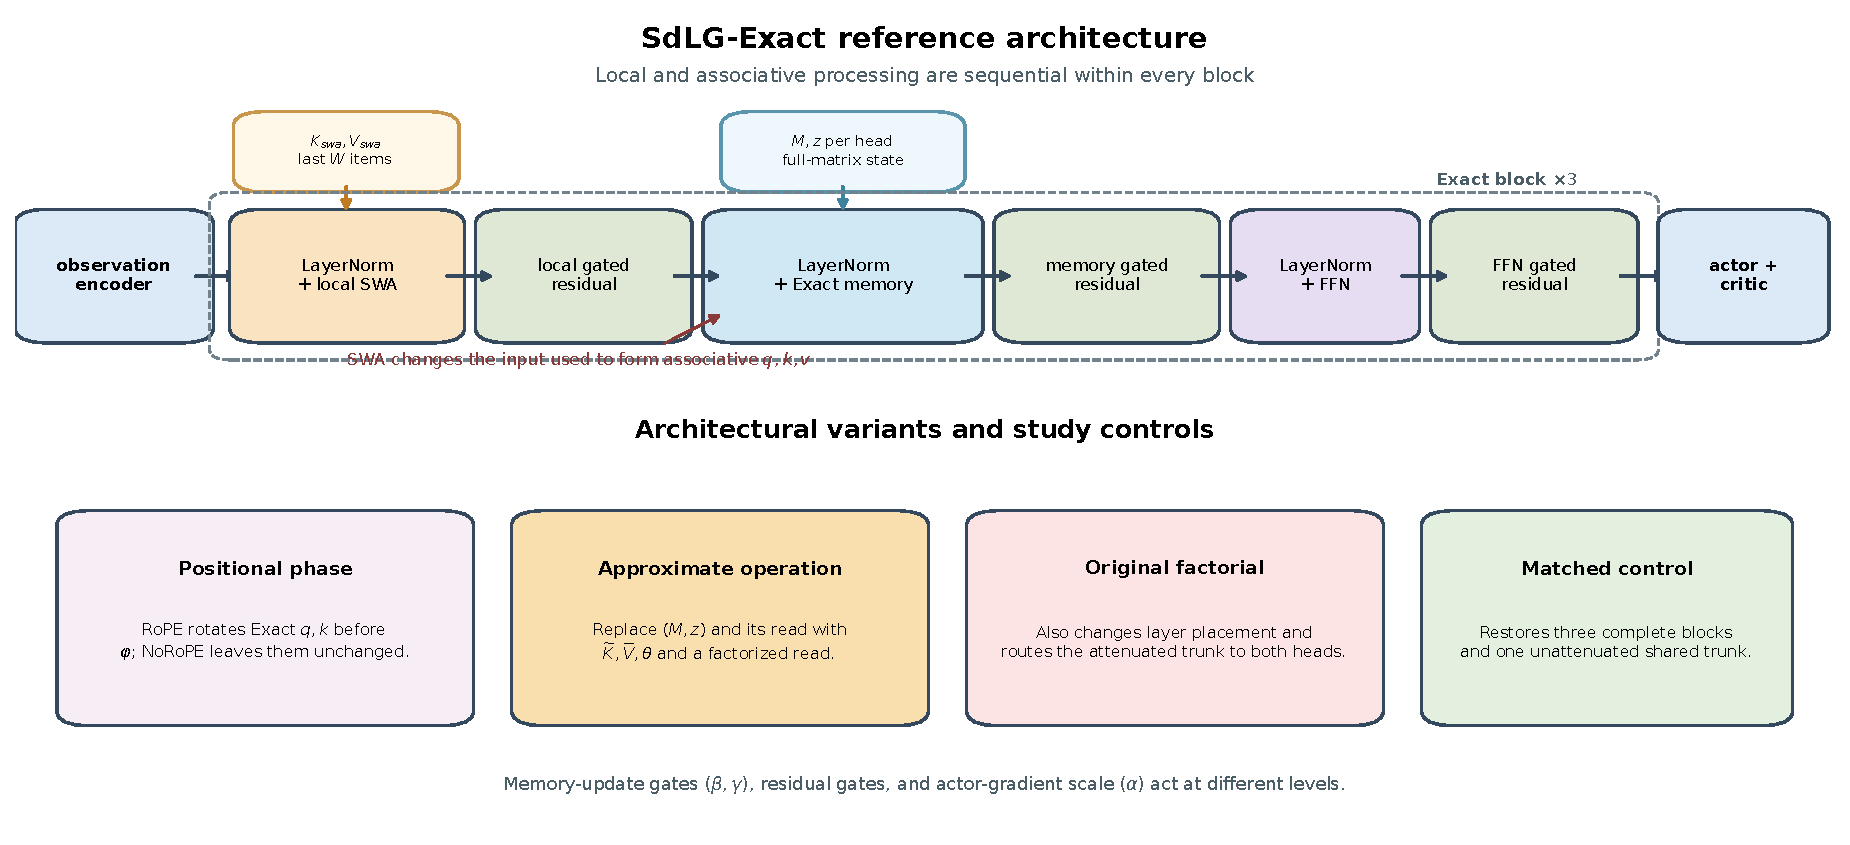
\includegraphics[width=0.92\textwidth]{plots/rebuilt/fig1_configuration_topologies}
\caption{\textbf{SdLG-Exact reference architecture and study-specific modifications.}
The large upper panel shows the implemented order within one Exact block:
pre-normalized SWA is fused by a gated residual, the full-matrix associative
stage reads and updates $(M,z)$ from the resulting representation and is fused
by a second gated residual, and an FFN is fused by a third. The tested T-Maze
reference repeats this complete block three times. The lower panel separates
modifications from the reference: positional phase changes query/key handling;
Approximate replaces the associative state, update, and read; the original
factorial also changes block placement and actor--critic routing; and the matched
comparison restores the reference block layout and common trunk.}
\label{fig:sdlg_flow}
\end{figure*}

\subsection{Reference Block and Processing Order}
Let $x_t^{(\ell)}$ denote the input to block $\ell$ at environment step $t$.
The block applies the following sequence:
\begin{align}
u_t^{(\ell)}
  &= \operatorname{SWA}\!\left(\operatorname{LN}(x_t^{(\ell)});
      K_{\mathrm{swa}},V_{\mathrm{swa}}\right),\\
x_{t,\mathrm{loc}}^{(\ell)}
  &= \mathcal{G}_{\mathrm{loc}}\!\left(x_t^{(\ell)},u_t^{(\ell)}\right),\\
(a_t^{(\ell)},M_t^{(\ell)},z_t^{(\ell)})
  &= \mathcal{A}_{\mathrm{Exact}}\!\left(\operatorname{LN}(x_{t,\mathrm{loc}}^{(\ell)});\right.\notag\\[-2pt]
  &\quad\left.M_{t-1}^{(\ell)},z_{t-1}^{(\ell)}\right),\\
x_{t,\mathrm{mem}}^{(\ell)}
  &= \mathcal{G}_{\mathrm{mem}}\!\left(x_{t,\mathrm{loc}}^{(\ell)},a_t^{(\ell)}\right),\\
f_t^{(\ell)}
  &= \operatorname{FFN}\!\left(\operatorname{LN}(x_{t,\mathrm{mem}}^{(\ell)})\right),\\
x_t^{(\ell+1)}
  &= \mathcal{G}_{\mathrm{ffn}}\!\left(x_{t,\mathrm{mem}}^{(\ell)},f_t^{(\ell)}\right).
\label{eq:exact_block_order}
\end{align}
Here $\mathcal{G}$ denotes a GTrXL-style GRU residual gate. The three gate
instances have separate parameters. The tested T-Maze Exact model applies three
of these complete blocks after a two-layer observation encoder, then sends the
final shared representation to the actor and critic heads.

This ordering resolves two different uses of the word \emph{parallel}. The
local and associative modules are sequential components of a block. Across the
time axis, however, the Exact affine recurrence is associative and can be
evaluated with a parallel prefix scan over a training chunk. Online execution
still updates it one environment step at a time.

\subsection{Local Sliding-Window Attention}
The local module stores $W$ projected key/value pairs and supplies a locally
processed residual stream to the associative recurrence. The execution used for the main results
uses circular buffer writes during one-step rollout and a chronological buffer
interpretation during sequence recomputation, without converting between the
two layouts. These paths therefore need not implement identical local windows.
Buffers carry across nonterminal rollout chunks and reset at episode boundaries;
the counter convention also distinguishes fresh initialization from an episode
reset. Appendix~\ref{app:original_local_execution} specifies these semantics.
The associative scan equivalence below concerns the associative recurrence for
given inputs, not equivalence of the entire policy across these execution paths.

\subsection{Gated Full-Matrix Associative Memory}
For each associative head, Exact maintains a matrix
$M_t\in\mathbb{R}^{d_k\times d_v}$ and a normalizer
$z_t\in\mathbb{R}^{d_k}$. From the locally processed representation it projects
$q_t,k_t\in\mathbb{R}^{d_k}$ and $v_t\in\mathbb{R}^{d_v}$, together with a scalar
write gate $\beta_t\in[0,1]$ and decay gate $\gamma_t\in(0,1]$. With the positive
feature map $\varphi(u)=1+\operatorname{ELU}(u)$, the state update is
\begin{align}
M_t &= \gamma_t M_{t-1}+\beta_t\varphi(k_t)v_t^\top,
\label{eq:matrix_recurrence}\\
z_t &= \gamma_t z_{t-1}+\beta_t\varphi(k_t),
\end{align}
and the query-dependent read is
\begin{equation}
y_t=\frac{\varphi(q_t)^\top M_t}
{\varphi(q_t)^\top z_t+\varepsilon},\qquad \varepsilon=10^{-6}.
\label{eq:query_retrieval}
\end{equation}
Exact therefore does not retain a list of all earlier keys and values or apply a
softmax over the full history. It retrieves from accumulated outer-product
associations, normalized by accumulated key features. Recall depends on the
learned representation, gate behavior, associative load, and interference. The
name \emph{Exact} identifies this full-matrix execution rather than promising
error-free recall or unlimited capacity. The implementation uses multiple
associative heads with separate matrix states and decay timescales.

At a new-episode observation, the continuation mask removes the preceding
episode's matrix and normalizer before the current write. Across a nonterminal
TBPTT boundary, $(M,z)$ and the SWA buffers are carried forward while their
computational graphs are detached. The associative composition proof, reset
semantics, and JAX implementation appear in Appendices~\ref{app:math_details}
and~\ref{app:implementation_details}.

\subsection{Three Distinct Control Mechanisms}
Three controls that act at different levels must not be conflated. First,
$\beta_t$ and $\gamma_t$ are \emph{memory-update gates}: they determine what is
written to the associative state and how much prior state is retained. Second,
$\mathcal{G}_{\mathrm{loc}}$, $\mathcal{G}_{\mathrm{mem}}$, and
$\mathcal{G}_{\mathrm{ffn}}$ are \emph{residual gates}: they determine how module
outputs alter the shared representation; they do not change Equations
\ref{eq:matrix_recurrence}--\ref{eq:query_retrieval}. Third, actor-gradient
routing is an \emph{optimization control} applied after the recurrent trunk. In
the dedicated Craftax Hybrid study it uses
\begin{equation}
x_{\mathrm{critic}}=x,\qquad
x_{\mathrm{actor}}=(1-\alpha)\operatorname{stopgrad}(x)+\alpha x,
\label{eq:ggs}
\end{equation}
so $\alpha$ scales the actor gradient entering the shared trunk without changing
the actor's forward input. It is not part of the Exact recurrence. SWA also
contains an internal output gate, but this belongs to the local module and is
separate from all three controls above.

\subsection{Controlled Modifications to the Reference}
The experiments change specific parts of the reference architecture:

\paragraph{Positional phase.}
When running-phase RoPE is enabled, the Exact branch rotates projected queries
and keys before applying $\varphi$; NoRoPE passes them through unchanged. This
changes positional handling, not the matrix state or the sequential block order.

\paragraph{Approximate associative execution.}
SdLG-Approximate replaces $(M,z)$ and Equations
\ref{eq:matrix_recurrence}--\ref{eq:query_retrieval} with factorized key and value
states $(\widetilde K,\widetilde V)$, phase state $\theta$, and a different
normalized read. It is therefore an alternative associative formulation, not
Exact with a smaller rank. Its equations and phase handling are given in
Appendix~\ref{app:approximate_execution}. Here $r$ is the total number of stored
factor rows per layer; Approximate has no Exact-style associative head axis and
shares its learned projections and update gates across rows. In the original T-Maze factorial,
Approximate additionally uses an alternating local--factorized--local stack and
routes an $\alpha=0.1$ attenuated representation to both PPO heads. That study
compares complete configurations rather than isolating associative rank. This
two-head attenuation differs from the actor-only gradient routing used in the
dedicated Craftax actor-gradient-scale study.

\paragraph{Matched execution control.}
The matched T-Maze comparison places Exact and Approximate associative operations
inside the same three complete local--associative--gated-FFN blocks and uses a
common unattenuated actor--critic trunk ($\alpha=1$). It removes block-placement
and routing differences while retaining the formulations' distinct state,
update, read, effective state size, and numerical path.

\paragraph{Component interventions.}
The MiniGrid intervention compares SWA enabled with SWA bypassed via
\texttt{local\_mode="none"}.
The Hybrid configuration is the factorized Approximate core with local
processing and a shared actor--critic trunk. The Craftax intervention changes
its actor-gradient scale. These are study-specific modifications, not defining
properties of Exact.

\section{Experimental Setup}
\label{sec:setup}

The experimental unit is a seeded training run or an independently seeded retrieval draw. We report seed-level outcomes for the small-sample studies, separate fixed endpoints from early stopping, and preserve right-censoring in T-Maze.

\subsection{Common Training and Evaluation Semantics}

We train recurrent policies with PPO and GAE over rollout chunks of length $T$~\cite{schulman2015high,schulman2017proximal}. State is carried but gradient-detached across nonterminal chunk boundaries and cleared at episode termination; Appendix~\ref{app:implementation_details} gives the equations and mask semantics.

The studies address complementary questions. DoorKey, POPGym, and the Craftax landscape provide cross-family task comparisons; T-Maze tests delayed retention across recurrent baselines and includes a controlled Exact--Approximate comparison. MemoryS16 and actor-gradient scaling are formulation-specific interventions, associative retrieval and corrective overwrite are synthetic diagnostics, and the matched state/latency and Craftax cross-$T$ studies characterize computational behavior. Appendix~\ref{app:repro_map} maps every study to its endpoint, seed coverage, and evidence.

\subsection{Passive T-Maze Retention Experiments}

\paragraph{Long-horizon state execution and phase.}
In Passive T-Maze~\cite{ni2023when}, a binary cue appears at reset and must be recalled at a decision junction at step $H$; matching one of two actions to the cue yields return 1, so an uninformed policy has expected return $0.5$. We compare the executed Exact and Approximate configurations with RoPE/NoRoPE at $H_{\mathrm{train}}=100$ under $T=16$, then evaluate $H=100,150,200$. Exact has three local--full-matrix-associative blocks; Approximate alternates local--factorized-associative--local and routes its $\alpha=0.1$ attenuated representation to both PPO heads. The factorial treats the four combinations as complete configurations.

Ten seeds per cell train up to 50M steps. A run stops after three consecutive logged training-episode mean returns reach $0.98$ or is right-censored; the resulting parameters are evaluated at $H=100,150,200$. Terminal step and endpoint returns are distinct.

For descriptive solve counts, a run is solved when terminal deterministic success over 256 episodes is at least $0.90$; an episode succeeds at return $\geq0.99$. This differs from the training stopping rule; return remains primary and threshold inference is post hoc and exploratory. The 200-step environment limit makes $H=200$ the largest valid evaluation horizon; longer horizons are untested.

\paragraph{Matched state execution.}
A matched control fixes the three-block local layout, NoRoPE, and common unattenuated actor--critic trunk ($\alpha=1$) while comparing full-matrix Exact with a factorized Approximate state having $r=16$ stored rows per layer. In NoRoPE, the symmetric cosine frequencies yield eight pairs of identical factor trajectories, so this configuration has at most eight distinct factor states in exact arithmetic. NoRoPE was selected after examining the factorial, where it was the best Exact phase setting, so the choice was not prospectively independent. The control uses ten independent runs per cell, with $H=200$ primary. Appendix~\ref{app:tmaze_matched_execution} records the configuration and checks.

\paragraph{Cross-family T-Maze baselines.}
We evaluate GRU, LSTM, Mamba, LTI-Linear, Markovian, GLA, GTrXL-64, and GTrXL-128 policies on Passive T-Maze at $H=100$ and $T=16$. Seven seeds per configuration use the same 50M-step cap, early-stopping rule, and terminal-policy evaluations at $H\in\{100,150,200\}$ as the SdLG studies. The model families differ in parameter count, and the studies use independent seed-level samples. Cross-family results therefore characterize the evaluated configurations rather than parameter-matched architecture effects. Appendix~\ref{app:tmaze_external_landscape} reports the outcomes and summaries.

\subsection{Component Interventions}

\paragraph{Local processing and shared-gradient coupling.}
Within the evaluated SdLG-Approximate formulation, XLand-MiniGrid's MemoryS16 environment~\cite{minigrid,nikulin2024xland} compares SWA enabled with SWA bypassed at a fixed endpoint. Each condition contains 15 runs, and uncertainty is estimated using an independent seed-level bootstrap.

The Craftax-Classic actor-gradient-scale study~\cite{matthews2024craftax} uses the Hybrid formulation and compares $\alpha=0.1$ and $1.0$ over five seeds at $T=64$ and 20,152,320 steps. Matched initializations, random-number streams, and evaluation seeds motivate paired resampling, although realized trajectories may diverge. Probe cosine is aggregated within seed before condition summaries and is not treated as a mediator.

\subsection{Independent Diagnostics and Benchmark Context}

\paragraph{Independent retrieval diagnostic.}
The controlled associative-retrieval factorial crosses load $N$, addressing dimension $d_k$, and value dimension $d_v$. It writes $N$ normalized associations into a delta-updated matrix state:
\begin{align}
\widehat v_t&=M_t^\top k_t,\qquad e_t=v_t-\widehat v_t,\\
M_{t+1}&=M_t+\frac{c}{\lVert k_t\rVert_2^2+10^{-5}}k_te_t^\top,
\label{eq:capacity_update}
\end{align}
with $M_0=0$ and fixed correction coefficient $c=0.125$. Each of the 48 cells contains ten draws; retrieval quality is the mean cosine similarity between each retrieved value and its target. The factorial characterizes finite-regime retrieval behavior of this synthetic recurrence, separately from policy optimization and environment feedback.
Here $k_t\in\mathbb{R}^{d_k}$ and $v_t\in\mathbb{R}^{d_v}$ are the normalized key and target value, $\widehat v_t$ is the current retrieval, $e_t$ is its correction error, and $M_t\in\mathbb{R}^{d_k\times d_v}$ is the memory state. The overwrite diagnostic below uses its reported coefficient $\eta$ directly and is a separate protocol.
This diagnostic does not execute SdLG-Exact: it omits Exact's learned decay and write gates, positive ELU feature map, normalizer state $z_t$, and normalized query read. It characterizes only the stated Delta recurrence.

\paragraph{Corrective overwrite diagnostic.}
A synthetic reassignment protocol tests the corrective-update motivation for fast weights~\cite{schlag2021linear}: it replaces one quarter of the stored values and measures target overwrite separately from non-target preservation. Additive memory, a fixed-gated proxy, and normalized Delta updates with $\eta\in\{0.25,0.5,1.0\}$ share ten draws per $(N,d_k,d_v)$ cell.

\paragraph{DoorKey cross-family evaluation.}
MiniGrid-DoorKey-8x8 compares SdLG-Exact, PPO-GRU, and PPO-GTrXL on seeds $\{42,54,99,123,456\}$ with a shared encoder, PPO settings, $512$ environments, and $T=64$. Training stops after three consecutive logged returns reach $0.96$, or at the 20M-step cap. Terminal stochastic-policy evaluation uses 256 episodes; success means positive return. We report five-run means, sample SDs, and early-stop/cap counts. Capacities differ (1.635M, 0.327M, and 0.969M parameters, respectively). This comparison does not test the MemoryS16 SWA intervention; Appendix~\ref{app:doorkey_8x8} gives run-level endpoints and evaluation seeds.

\paragraph{Cross-architecture and systems comparisons.}
The matched state/latency measurement evaluates the two constructions at batches 1 and 256 using 300 synchronized timings after 50 warmups; timings are replicates, not trained-policy seeds. The capacity-unmatched Craftax comparison uses $T=64$ and 50M steps: returns are final logged training-episode means and SPS covers the full training loop. A five-seed cross-$T$ experiment reports cells at $T\in\{16,32,64,128\}$. Because $T$ also changes GAE and PPO update structure, this is a configuration response. The POPGym evaluation suite~\cite{morad2023popgym} covers 16 Easy and 7 Medium tasks; Appendix~\ref{app:experiment_protocols} specifies task-specific model, seed, endpoint, and remaining provenance coverage.

\section{Results}
\label{sec:results}

We report task-dependent architecture behavior, delayed retention, associative retrieval and updating, component interventions, and training/execution cost under the estimands defined in Section~\ref{sec:setup}.

\subsection{Delayed Retention on Passive T-Maze}
\label{sec:tmaze_extrapolation}
How do recurrent architectures behave at the trained horizon and at longer unseen delays? We first compare established recurrent families with SdLG, then examine within-family behavior through the execution-by-phase factorial and the topology-matched formulation control.

\paragraph{Cross-family baselines.}
Table~\ref{tab:tmaze_external_main} reports terminal-policy evaluations for seven seeds of each baseline.

\begin{table*}[t]
\centering\footnotesize
\setlength{\tabcolsep}{3.5pt}
\caption{\textbf{Passive T-Maze cross-family baselines.} Mean $\pm$ sample SD over seven seeds. E/C counts early stops versus cap outcomes. Parameter counts are contextual; terminal steps do not replace horizon return.}
\label{tab:tmaze_external_main}
\begin{tabular}{lrrrrrr}
\toprule
Model & Parameters & E/C & Terminal steps (M) & $H=100$ & $H=150$ & $H=200$ \\
\midrule
GRU         & 116,227   & 1/6 & $49.012\pm2.539$ & $0.644\pm0.243$ & $0.426\pm0.345$ & $0.574\pm0.188$ \\
LSTM        & 148,995   & 0/7 & $49.971\pm0.000$ & $0.571\pm0.189$ & $0.503\pm0.008$ & $0.433\pm0.191$ \\
Mamba       & 132,611   & 0/7 & $49.971\pm0.000$ & $0.499\pm0.008$ & $0.499\pm0.008$ & $0.499\pm0.008$ \\
LTI-Linear  &  66,691   & 0/7 & $49.971\pm0.000$ & $0.501\pm0.008$ & $0.501\pm0.008$ & $0.501\pm0.008$ \\
Markovian   &  50,435   & 0/7 & $49.971\pm0.000$ & $0.506\pm0.006$ & $0.506\pm0.006$ & $0.506\pm0.006$ \\
GLA         & 1,208,195 & 7/0 & $ 5.337\pm3.852$ & $0.782\pm0.271$ & $0.782\pm0.271$ & $0.710\pm0.271$ \\
GTrXL-64    &   956,547 & 7/0 & $ 5.781\pm2.349$ & $0.930\pm0.186$ & $0.501\pm0.008$ & $0.501\pm0.008$ \\
GTrXL-128   &   956,547 & 7/0 & $ 1.428\pm0.310$ & $1.000\pm0.000$ & $0.574\pm0.188$ & $0.503\pm0.008$ \\
\bottomrule
\end{tabular}
\par\smallskip\raggedright\footnotesize
\textit{For reference,} the independently evaluated ten-seed Matched Exact condition reaches $0.900\pm0.211$, $0.900\pm0.211$, and $0.851\pm0.240$ at $H=100,150,200$, respectively (Appendix Table~\ref{tab:tmaze_overview}). These runs use a different seed set from the seven-seed baselines.
\end{table*}

GRU and LSTM show inconsistent training-horizon learning: one GRU and no LSTM runs stop early, although both $H=100$ means exceed chance. Mamba, LTI-Linear, and Markovian remain near chance. At the trained horizon $H=100$, both GTrXL configurations have higher observed means than Matched Exact: $0.930$ for GTrXL-64 and $1.000$ for GTrXL-128, versus $0.900$ for Exact. At the unseen $H=200$, the GTrXL means fall to approximately chance, whereas Matched Exact retains $0.851$; GLA has the highest baseline mean there ($0.710$).

\paragraph{Execution-by-phase factorial.}
Exact-NoRoPE reaches mean returns $0.900$, $0.900$, and $0.851$ at $H=100,150,200$; both Approximate conditions are near $0.50$ at $H=200$. The marginal Exact-minus-Approximate contrast is $0.251$ with a 95\% percentile-bootstrap interval $[0.151,0.351]$ at $H=200$ (Figure~\ref{fig:tmaze_factorial}).

\begin{figure*}[t]
\centering
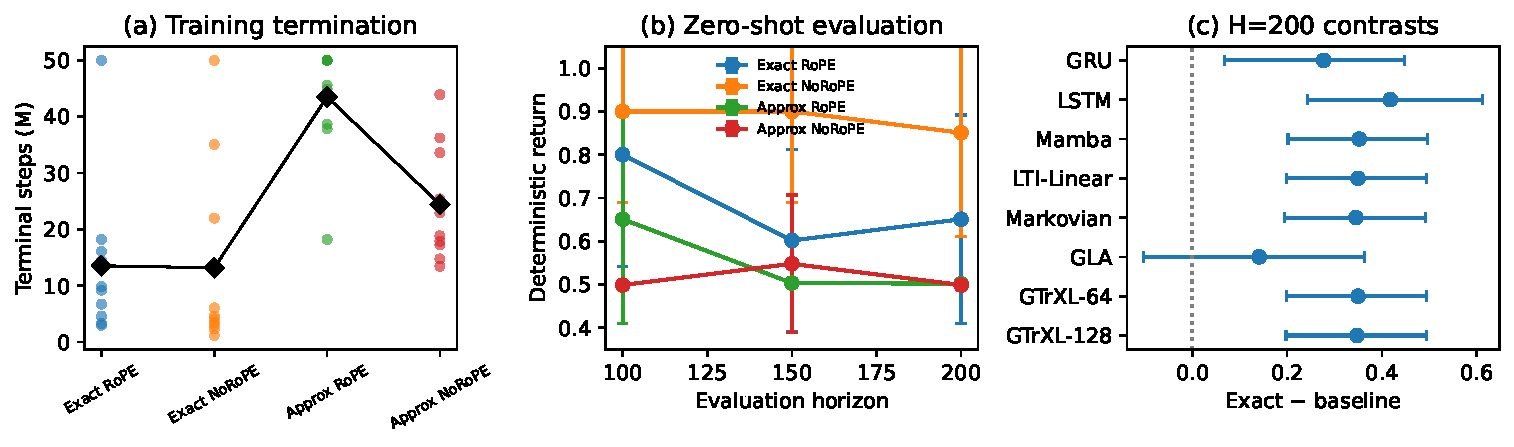
\includegraphics[width=0.74\textwidth]{plots/rebuilt/fig3_tmaze_rank_rope}
\caption{\textbf{State execution $\times$ positional phase on Passive T-Maze.} (a) Terminal steps; triangles denote capped runs, circles early stops, and bars mean $\pm$ SD. (b) Ten-seed mean return; Appendix Table~\ref{tab:tmaze_overview} gives SDs. (c) Independent-seed Exact-minus-Approximate $H=200$ contrasts; whiskers are 95\% percentile-bootstrap intervals.}
\label{fig:tmaze_factorial}
\end{figure*}

\paragraph{Matched execution.}
In the matched control, Exact reaches $0.851$ at the primary $H=200$ endpoint versus $0.500$ for Approximate, a difference of $0.351$ with a 95\% percentile-bootstrap interval $[0.200,0.497]$ (Figure~\ref{fig:tmaze_factorial}c). The comparison concerns the complete formulations rather than rank alone.

At $H=200$, the documented solve criterion classifies 7/10 Exact-NoRoPE and 0/10 Approximate-NoRoPE runs as solved in both the original factorial and matched study. Return remains primary; Appendix Table~\ref{tab:tmaze_solve_exploratory} gives post hoc exploratory Wilson intervals and Fisher tests. Early stops and terminal solves use different rollouts and thresholds and need not agree.

\subsection{Independent Associative-Memory Diagnostics}
\label{sec:results_associative}
The retrieval factorial tests a normalized Delta-rule system, while the reassignment study compares additive, fixed-gated-proxy, and normalized Delta updates on shared random associations.

\paragraph{Retrieval under associative load.}
The retrieval factorial contains ten draws in each of 48 cells over the $N,d_k,d_v$ grid defined in Section~\ref{sec:setup}.
Retrieval increases monotonically with $d_k$ in every draw at every tested load, while the $d_v$ marginal spans only $0.002$--$0.010$. It also declines systematically as $N/d_k$ grows from $0.25$ to $8$ (Figure~\ref{fig:associative_capacity}). Equal-$N/d_k$ configurations are close but not identical, with a maximum mean spread of $0.013$.

\begin{figure}[t]
\centering
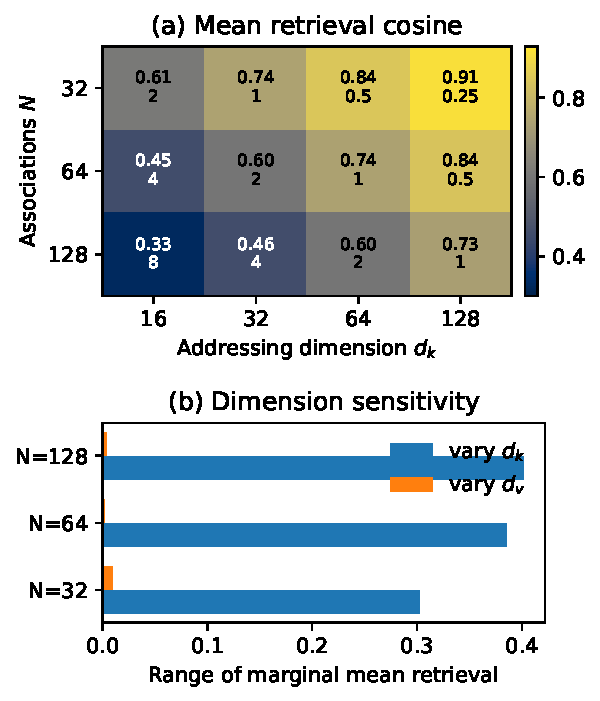
\includegraphics[width=0.78\linewidth]{plots/rebuilt/fig6_associative_capacity}
\caption{\textbf{Normalized Delta-rule retrieval diagnostic.} (a) Mean cosine by $(N,d_k)$ over $d_v$ and ten draws; sublabels give $N/d_k$. (b) Marginal ranges show greater addressing-dimension sensitivity.}
\label{fig:associative_capacity}
\end{figure}

Thus the synthetic recurrence is empirically more sensitive to addressing than value dimension under the tested random-association distribution and loads. The worst-case rank bound does not quantify this sensitivity or the capacity of learned SdLG-Exact (Appendix~\ref{app:capacity_bound_sec}).

\paragraph{Corrective reassignment.}
Does a corrective update improve replacement without damaging untouched associations? Relative to additive memory, normalized Delta updates at $\eta=0.25$ raise target fidelity from $0.502$ to $0.685$, a paired fixed-grid difference of $0.183$ with a 95\% within-cell paired-bootstrap interval $[0.181,0.185]$. Increasing $\eta$ from $0.25$ to $1.0$ adds $0.124$ in target fidelity (95\% interval $[0.122,0.127]$) but reduces non-target preservation by $0.160$ (95\% interval $[0.158,0.162]$). Stronger correction therefore improves reassignment at a measurable cost to untouched associations under this protocol. The fixed-gated proxy and complete method table appear in Appendix~\ref{app:component_transfer}.

\subsection{Task-Dependent Architecture Ordering}
\label{sec:popgym_results}
\paragraph{DoorKey-8x8 comparison.}
Across five seeds per model, Exact has the highest mean terminal return and success rate and the most early stops (three versus two for GTrXL and one for GRU; Table~\ref{tab:doorkey_8x8_main}).

\begin{table}[t]
\centering\footnotesize
\setlength{\tabcolsep}{3pt}
\caption{\textbf{DoorKey-8x8 terminal-policy evaluation.} Five-seed mean $\pm$ sample SD; E/C counts early stops versus caps. Appendix~\ref{app:doorkey_8x8} gives individual runs.}
\label{tab:doorkey_8x8_main}
\begin{tabular}{lrrr}
\toprule
Model & Eval. return & Success rate & E/C \\
\midrule
SdLG-Exact & $0.668\pm0.408$ & $0.748\pm0.362$ & 3/2 \\
PPO-GRU & $0.193\pm0.432$ & $0.200\pm0.447$ & 1/4 \\
PPO-GTrXL & $0.468\pm0.466$ & $0.537\pm0.446$ & 2/3 \\
\bottomrule
\end{tabular}

\end{table}

\paragraph{POPGym task comparisons.}
The POPGym evaluations~\cite{morad2023popgym} use each seed's maximum logged evaluation return, with three seeds for the multi-seed task comparisons discussed here. Exact exceeds GRU on CountRecall (accumulation/query) but is lower on Concentration (discrete matching), MinesweeperEasy ($0.591$ versus $0.942$), and LabyrinthEscapeEasy ($0.671$ versus $0.971$; Appendix Table~\ref{table:popgym_easy_full}). The two SdLG formulations also change order by task: Exact exceeds Approximate on CountRecallEasy ($0.670$ versus $-0.712$), whereas Approximate is higher on ConcentrationEasy ($-0.102$ versus $-0.267$) and LabyrinthEscapeEasy ($0.967$ versus $0.671$; Appendix Table~\ref{table:popgym_easy_full}).

\subsection{Component Interventions}
\label{sec:optional_controls}

\paragraph{Local pathway in SdLG-Approximate.}
On XLand-MiniGrid MemoryS16, SWA enabled has mean return $0.508$ (SD $0.445$), versus $0.782$ (SD $0.354$) when bypassed; the enabled-minus-bypassed difference is $-0.274$ with a 95\% independent-bootstrap interval $[-0.549,0.008]$ over 15 runs per condition (Appendix Figure~\ref{fig:minigrid_ablation}). The interval includes zero.

\paragraph{Actor-gradient scaling in the Hybrid configuration.}
At 20.15M steps, $\alpha=0.1$ has mean return $11.210$ versus $9.757$ for $\alpha=1.0$. All five matched pairs favor attenuation (Figure~\ref{fig:ggs_telemetry}); the paired difference is $1.453$ with a 95\% percentile-bootstrap interval $[0.925,1.962]$. This interval is conditional on the five observed pairs; with five pairs, the smallest attainable two-sided exact sign-flip $p$-value is $0.0625$. Probe cosine remains descriptive rather than a PPO-loss-conflict measure.

\begin{figure}[t]
\centering
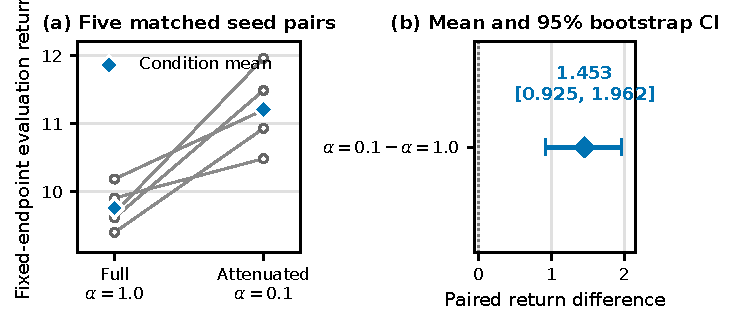
\includegraphics[width=0.70\linewidth]{plots/gradient_shielding_paired.pdf}
\caption{\textbf{Actor-gradient scale on Craftax.} (a) Five matched-seed endpoint returns; lines join common initializations and random streams, and diamonds mark means. (b) Attenuated-minus-full paired mean and exact percentile-bootstrap 95\% interval.}
\label{fig:ggs_telemetry}
\end{figure}

\subsection{Training-Configuration and Systems Behavior}
\label{sec:systems_results}

\paragraph{Rollout/TBPTT-length response.}
Do architecture orderings depend on the rollout/TBPTT configuration?
The Craftax cross-$T$ results report five-run final logged training-return means after a 50M-step budget (Figure~\ref{fig:craftax_cross_t}). SdLG-Approx changes from $16.33\pm0.37$ at $T=16$ to $14.79\pm0.36$ at $T=64$, while PPO-GLA reaches $15.69\pm0.22$ at $T=64$. Ordering varies with $T$, which jointly changes rollout, TBPTT, GAE, and update structure.

\begin{figure}[t]
\centering
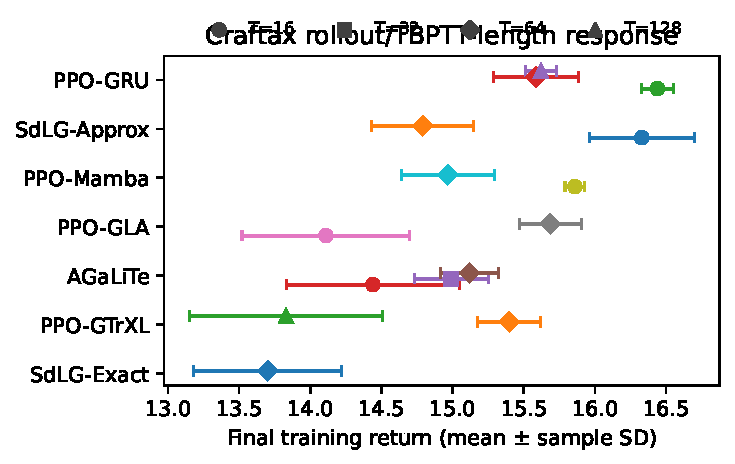
\includegraphics[width=0.72\linewidth]{plots/rebuilt/fig7_craftax_cross_t.pdf}
\caption{\textbf{Craftax rollout/TBPTT-length response.} Five-run final logged training-return mean $\pm$ SD after a 50M-step budget. Markers identify rollout/TBPTT length $T$; blank cells were not run. SdLG-Approx is logged as \texttt{SdLGHybrid} with a coupled trunk.}
\label{fig:craftax_cross_t}
\end{figure}

\paragraph{Fixed-$T$ return and training-loop throughput.}
At $T=64$ and 50M steps, PPO-GRU ($0.81$M parameters) reaches return $15.59$ and 25.2k loop steps/s; the other four models span $14.97$--$15.69$ and 10.0k--17.8k steps/s. Exact reaches $13.70\pm0.52$ across five runs; its measured cumulative training-loop throughput is approximately 9.4k environment steps/s. These are cumulative loop measurements, not recurrent-step latency or kernel throughput.

\paragraph{Matched recurrent-state and inference cost.}
Under a matched three-block topology, Approximate carries 24,780 bytes per environment versus 62,988 for Exact, a $60.7\%$ reduction. Median warmed latency is $0.984$ versus $0.960$ ms at batch 256 and $0.675$ versus $0.586$ ms at batch 1 (300 iterations after 50 warm-ups on ROCm). Factorization saves state without reducing latency; bytes exclude parameters, activations, and allocation overhead (Appendix~\ref{app:component_transfer}).

\balance
\section{Design Implications and Operating Boundaries}
\label{sec:discussion}

The results address the research question along three dimensions: where the tested mechanisms help, where they fail to help, and what they cost.

The protocols separate seeded task-level evaluations from controlled memory-operation diagnostics and systems measurements. Matched controls narrow configuration differences, whereas cross-family benchmarks provide broader capacity-unmatched context; each result is therefore interpreted according to its endpoint and controls.

\paragraph{Evaluate retention, retrieval, and revision as separate capabilities.}
Across T-Maze, DoorKey, POPGym, and Craftax, observed architecture orderings depend on the task, horizon, configuration, and evaluation metric. GTrXL performs strongly at the trained T-Maze horizon but deteriorates at longer unseen delays; Exact has the highest observed mean in the reported DoorKey comparison, while POPGym and Craftax favor other architectures in several settings. Internal SdLG formulation controls provide additional evidence that execution choices can substantially alter behavior. These comparisons characterize the tested operating regimes without establishing general architectural superiority.

\paragraph{Evaluate memory and compute efficiency separately.}
Carried-state size, warmed recurrent-step latency, and end-to-end loop SPS measure different costs. Factorization reduces carried state here without reducing measured one-step latency, while loop SPS also includes environment interaction, optimization, data movement, and logging. Efficiency claims must therefore name both the metric and implementation context.

\paragraph{Validate components in each configuration.}
The SWA and actor-gradient studies test different formulations and tasks; their results do not define context-independent component effects. Components therefore require evaluation in each task and architecture.

\paragraph{Limitations.}
The matched Exact--Approximate comparison does not isolate a single architectural change. Matched NoRoPE selection followed the factorial and was not prospectively independent. Cross-family T-Maze results compare the evaluated configurations rather than parameter-matched architectures. The available compute budget constrained seed counts and the breadth of cross-family tuning and Exact-specific component studies. Intervals are unadjusted, solve analyses exploratory, and $H>200$ untested. Approximate/Hybrid interventions need not transfer to Exact. The actor-gradient study has five pairs. POPGym and Craftax compare models of different capacities.

\section{Conclusion}
No single recurrent architecture leads across all evaluated tasks and operating conditions. GTrXL, Exact, GRU, GLA, Mamba, and Approximate exhibit different observed strengths across memory demands, horizons, and computational constraints. The synthetic diagnostics separate addressing sensitivity from the replacement--preservation trade-off, while the component interventions show configuration-dependent effects. Factorization reduces carried state but not measured latency, and Exact has the lowest measured Craftax training-loop throughput. The contribution is an empirical account of the tested operating boundaries.


\FloatBarrier
\clearpage
\bibliography{references}
\bibliographystyle{icml2026}

\newpage
\newpage
\appendix
\onecolumn
\raggedbottom
\renewcommand{\theHsection}{app.\Alph{section}}
\renewcommand{\theHtable}{app.tbl.\thesection.\arabic{table}}
\renewcommand{\theHfigure}{app.fig.\thesection.\arabic{figure}}
\icmltitle{Appendix: Operational Memory Study Supplement \& Reproduction Manual}
\numberwithin{table}{section}
\numberwithin{figure}{section}

%%%%%%%%%%%%%%%%%%%%%%%%%%%%%%%%%%%%%%%%%%%%%%%%%%%%%%%%%%%%%%%%%%%%%%%%%%%%%%%
% APPENDIX A: Reproducibility Roadmap & Master Experiment Mapping
%%%%%%%%%%%%%%%%%%%%%%%%%%%%%%%%%%%%%%%%%%%%%%%%%%%%%%%%%%%%%%%%%%%%%%%%%%%%%%%
\section{Reproducibility Roadmap \& Master Experiment Mapping}
\label{app:repro_map}

This appendix preserves extended results, configurations, implementation detail, and reproduction material supporting the main-text experiments.

Each main-text result maps to an experiment ID, evaluation protocol, and evidence in Table~\ref{table:repro_roadmap}.

\paragraph{Code and evidence.}
The standalone supplementary repository contains the supported release commands, versioned configurations, compact result records, and source artifacts named below. Run commands from the repository root through \texttt{scripts/reproduce.py}; the frozen records and generated artifacts are checked by the release audit. Study-specific limits on fresh heavyweight reproduction are reported with the corresponding protocols.

\begin{table*}[htbp]
\caption{\textbf{Experiment and evidence map.} Paper results, experiment IDs, protocols, and evidence. Protocol details are in Appendix~\ref{app:experiment_protocols}; commands are in Appendix~\ref{app:repro_checklist}. POPGym records retain task-specific seed coverage and endpoints.}
\label{table:repro_roadmap}
\vskip 0.1in
\begin{center}
\begin{small}
\setlength{\tabcolsep}{4pt}
\begin{tabularx}{\linewidth}{@{}
    >{\raggedright\arraybackslash}p{0.12\textwidth}
    >{\raggedright\arraybackslash}p{0.19\textwidth}
    >{\raggedright\arraybackslash}p{0.145\textwidth}
    >{\raggedright\arraybackslash}p{0.11\textwidth}
    >{\raggedright\arraybackslash}X@{}}
\toprule
\textbf{Paper Result} & \textbf{Study / Environment} & \textbf{Budget / Protocol} & \textbf{Seed Coverage} & \textbf{Experiment ID / Evidence} \\
\midrule
\S 5.5 / App D & Craftax-Classic & 50M steps; $T\in\{16,32,64,128\}$ & 5/run cell & \shortstack[l]{\texttt{T3-CRAFTAX-}\\\texttt{CROSS-T}\\Final logged training-return\\summaries} \\
Fig. 2 / \S 5.1 & Passive T-Maze & $\leq50$M steps; $T=16$ & 10 & \shortstack[l]{\texttt{T1-TMAZE-}\\\texttt{EXECUTION-PHASE}\\Terminal-step and\\horizon-return records} \\
\S 5.1 / App D & Passive T-Maze & $\leq50$M steps; $T=16$ & 10/cell & \shortstack[l]{\texttt{T1-TMAZE-MATCHED-}\\\texttt{EXECUTION}\\Matched horizon-return records} \\
\S 5.1 / App D & Passive T-Maze reference & $\leq50$M; common stop rule; $H=100$, $T=16$ & 7/family & \shortstack[l]{\texttt{T3-TMAZE-EXTERNAL-}\\\texttt{LANDSCAPE}\\Terminal-policy horizon records} \\
App. Fig.~\ref{fig:minigrid_ablation} / \S 5.4 & MiniGrid-MemoryS16 & 9.83M steps; $T=64$ & 15/condition & \shortstack[l]{\texttt{T1-MINIGRID-}\\\texttt{LOCAL-WINDOW}\\Endpoint returns per condition} \\
\S 5.3 / App.~\ref{app:doorkey_8x8} & MiniGrid-DoorKey-8x8 & $\leq20$M steps; $T=64$ & 5/model & \shortstack[l]{\texttt{T3-MINIGRID-}\\\texttt{DOORKEY-8X8}\\Terminal-policy evaluation} \\
\S 5.3 / App E & POPGym (23 tasks) & task-specific & per cell & \shortstack[l]{\texttt{T3-POPGYM-SUITE}\\Per-seed task records} \\
App.~\ref{app:minesweeper_ablation} & Minesweeper & 15M steps; $T=64$ & 3 & \shortstack[l]{\texttt{T3-MINESWEEPER-}\\\texttt{STRUCTURAL-SCOPE}\\Structural-scope results} \\
Fig.~\ref{fig:ggs_telemetry} / \S 5.4 & Craftax / telemetry & 20.15M steps; $T=64$ & 5 matched & \shortstack[l]{\texttt{T1-CRAFTAX-ACTOR-}\\\texttt{GRADIENT-SCALE}\\Paired endpoints and probe telemetry} \\
Fig. 3 / \S 5.2 & Delta-Rule retrieval & 480 draws & 10/cell & \shortstack[l]{\texttt{T2-ASSOCIATIVE-}\\\texttt{CAPACITY}\\Seeded retrieval draws} \\
\S 5.2 / App.~\ref{app:component_transfer} & Associative overwrite & 2,400 synthetic outcomes & 10/shared cell & \shortstack[l]{\texttt{CTV-A1-ASSOCIATIVE-}\\\texttt{OVERWRITE}\\Target and non-target\\retrieval records} \\
\S 5.5 / App.~\ref{app:component_transfer} & Matched state accounting & warmed recurrent step & 300 timings/cell & \shortstack[l]{\texttt{CTV-B2-MATCHED-}\\\texttt{STATE-INFERENCE}\\Carry-size and latency records} \\
\bottomrule
\end{tabularx}
\end{small}
\end{center}
\end{table*}

\subsection{Hardware \& Compute Environment Specifications}
The environment record names an AMD Radeon RX 6800 XT (16GB VRAM) workstation. The reported Craftax SPS values are cumulative training-loop measurements from the $T=64$ runs; they are not generalized to every study or interpreted as kernel throughput. The software versions below apply to those runs rather than the entire paper.
\begin{itemize}
    \item \textbf{Framework Stack:} Python v3.10, JAX v0.4.25, Flax v0.8.0, Optax v0.1.7, ROCm.
\end{itemize}

%%%%%%%%%%%%%%%%%%%%%%%%%%%%%%%%%%%%%%%%%%%%%%%%%%%%%%%%%%%%%%%%%%%%%%%%%%%%%%%
% APPENDIX B: Universal Experimental & Protocol Standards
%%%%%%%%%%%%%%%%%%%%%%%%%%%%%%%%%%%%%%%%%%%%%%%%%%%%%%%%%%%%%%%%%%%%%%%%%%%%%%%
\section{Cross-Experiment Semantics and Protocol Rules}
\label{app:protocol_standards}

The experiments share reporting semantics, while model and task settings remain study-specific. Only settings documented for each study are reported.

\subsection{Training Protocol Rules}
\begin{enumerate}
    \item \textbf{PPO Implementation Standard:} All models are trained using Proximal Policy Optimization (PPO) \cite{schulman2017proximal} built upon vectorized JAX environment rollouts. Advantage estimation uses Generalized Advantage Estimation (GAE) with $\gamma_{\mathrm{RL}} = 0.99$ and $\lambda_{\mathrm{GAE}} = 0.95$.
    \item \textbf{Rollout Truncation ($T$):} The T-Maze studies use $T=16$; MiniGrid, GGS, and Minesweeper use $T=64$. The Craftax cross-$T$ block has results at $T\in\{16,32,64,128\}$, while its fixed-$T$ systems comparison uses $T=64$. Backpropagation Through Time (BPTT) is truncated past the study-specific $T$.
    \item \textbf{Lifelong Recurrent Carry \& Stop-Gradient Barrier:} Each recurrent family carries its model-specific state $\mathcal{C}^{(\mathrm{model})}_t$ across nonterminal environment rollouts and detaches it at TBPTT boundaries. Exact SdLG carries $(M_t,z_t)$ plus local-window buffers and a step count; Approximate SdLG carries factorized key/value state, phase coordinates, and local-window buffers. PPO-GRU, PPO-GLA, and PPO-Mamba use their respective hidden states. Detachment prevents gradients from propagating past the chunk boundary while preserving forward context.
    \item \textbf{Shared Width/Depth Configuration ($d_{\text{model}}=256, N_{\text{layers}}=4$):} Craftax families use the same configured width and depth where applicable and share the same 2-layer MLP state encoder ($1335 \to 256 \to 256$) and actor/critic heads. Their instantiated totals nevertheless range from roughly $0.81\text{M}$ to $8.78\text{M}$ parameters. These comparisons are protocol-matched, not capacity-matched.
    \item \textbf{Identity-Biased Residual Gates:} The SdLG configurations use the fixed scalar offset $b_g=+2.0$, giving $z_0\approx0.12$ under zero pre-activation and initially biasing residual updates toward the identity stream. This is a configuration detail, not a universal setting.
\end{enumerate}

\subsection{Evaluation \& Statistical Protocol Rules}
\begin{enumerate}
    \item \textbf{Evaluation Horizons ($H_{\text{eval}}$):} The original factorial and matched T-Maze study train at $H=100$ and evaluate endpoint parameters at $H=100,150,200$. Other studies retain their task-native endpoint semantics.
    \item \textbf{Policy Execution:} T-Maze factorial evaluation uses deterministic actions over 256 evaluation environments. Craftax architecture benchmarks report training-episode return; GGS and MiniGrid use their stated evaluation protocols. POPGym uses the task-specific evaluation semantics stored with each result.
    \item \textbf{Statistical Aggregation:} Means and sample standard deviations use seeded runs as the experimental unit unless stated otherwise. T-Maze and MiniGrid contrasts use independent-condition resampling; GGS uses paired resampling of its five matched seeds. Reported intervals are pointwise and unadjusted. POPGym uses task-specific seed coverage; MMER denotes the maximum, over logged epochs, of the mean episodic reward at each epoch~\citep{morad2023popgym}. Study-specific endpoints and resampling details appear with each experiment.
\end{enumerate}

\section{Study-Specific Model Configurations}
\label{app:model_configs}

Architecture settings below are study-specific; there is no paper-wide default SdLG configuration. Values come from the corresponding experiment records.

\subsection{Experiment Identifiers \& Code Artifacts}
\begin{itemize}
    \item \texttt{CFG-CRAFTAX-MAIN}: Craftax 50M macro benchmark \\
    \textit{Script:} \path{scripts/diagnostics/benchmarks/craftax_full/craftax_classic_benchmark.py} \\
    \textit{Hyperparams:} $d_{\text{model}}=256, T=64, N_{\text{envs}}=256, \text{LR}=2\times 10^{-4}$.

    \item \texttt{T3-CRAFTAX-EXTERNAL-LANDSCAPE}: Craftax return and throughput evaluation \\
    \textit{Script:} \path{scripts/diagnostics/benchmarks/craftax_full/craftax_classic_benchmark.py} \\
    \textit{Hyperparams:} $d_{\text{model}}=256, T=64, N_{\text{envs}}=256, \text{LR}=2\times 10^{-4}$; five model families at endpoint 49,971,200.

    \item \texttt{T3-CRAFTAX-CROSS-T}: 50M Craftax rollout/TBPTT-length comparison \\
    \textit{Evidence:} Table~\ref{tab:app_craftax_returns} reports five-run endpoint-return summaries for the available $T\in\{16,32,64,128\}$ cells. \texttt{SdLGHybrid} is the logged runner name for SdLG-Approx with a coupled actor--critic trunk.
    
    \item \texttt{T1-TMAZE-EXECUTION-PHASE}: Passive T-Maze execution $\times$ phase factorial \\
    \textit{Script:} \path{scripts/diagnostics/exact_sdlg/exact_sdlg_tmaze_ablations.py} \\
    \textit{Hyperparams:} $d_{\text{model}}=128$, 3 layers, $d_k=d_v=32$, Exact with 4 associative heads, Approximate with $r=16$ total stored rows, $W=16$, $T=16$, $H_{\mathrm{train}}=100$, $N_{\text{envs}}=1024$, $\text{LR}=5\times10^{-4}$, ten seeds.

    \item \texttt{T1-TMAZE-MATCHED-EXECUTION}: topology- and gradient-matched state execution \\
    \textit{Script:} \path{scripts/diagnostics/exact_sdlg/exact_sdlg_tmaze_ablations.py} \\
    \textit{Hyperparams:} 3 local--associative--gated-FFN blocks, $d_{\text{model}}=128$, $d_k=d_v=32$, Exact with 4 associative heads, Approximate with $r=16$ total stored rows, $W=16$, NoRoPE, $\alpha=1$, $T=16$, $H_{\mathrm{train}}=100$, $N_{\text{envs}}=1024$, $\text{LR}=5\times10^{-4}$, ten seeds per condition.
    
    \item \texttt{T1-MINIGRID-LOCAL-WINDOW}: MiniGrid local-window ablation \\
    \textit{Script:} \path{scripts/diagnostics/architecture/swa_ablation/swa_ablation.py} \\
    \textit{Hyperparams:} $d_{\text{model}}=128$, 3 layers, 4 heads, $d_k=d_v=32$, $r=4$, $T=64$, $N_{\text{envs}}=256$, $\text{LR}=3\times10^{-4}$.
    
    \item \texttt{T3-POPGYM-SUITE}: POPGym task-native benchmark suite \\
    \textit{Implementation family:} \path{scripts/diagnostics/exact_sdlg/popgym_benchmark.py} \\
    \textit{Evidence:} 16 Easy and 7 Medium tasks with per-cell seed coverage, endpoints, and task-native MMER.
    
    \item \texttt{T1-CRAFTAX-ACTOR-GRADIENT-SCALE}: Gradient Gating Scale intervention \\
    \textit{Script:} \path{scripts/diagnostics/architecture/gradient_shielding/gradient_shielding.py} \\
    \textit{Hyperparams:} $d_{\text{model}}=256$, 4 layers, 8 heads, $d_k=d_v=32$, $r=4$, $W=8$, $T=64$, $N_{\text{envs}}=256$, $\alpha\in\{0.1,1.0\}$, $\text{LR}=3\times10^{-4}$.
\end{itemize}

\subsection{PPO-GRU}
\begin{itemize}
    \item \textbf{Architecture:} Gated Recurrent Unit~\cite{cho2014learning}; width and task heads follow the study record.
    \item \textbf{Parameters:} 809,234 in the Craftax actor--critic tree; task-specific POPGym checkpoint trees contain 119,580 parameters on \texttt{CountRecallEasy} and 148,917 on \texttt{ConcentrationEasy}.
    \item \textbf{State Carry:} The hidden vector carries across nonterminal chunks and resets on episode termination.
\end{itemize}

\subsection{PPO-Mamba}
\begin{itemize}
    \item \textbf{Architecture:} Selective State-Space Model~\cite{gu2023mamba} with $d_{\text{state}}=16$, convolutional width $d_{\text{conv}}=4$, and standardized hidden dimension $d_{\text{model}}=256$ ($N_{\text{layers}}=4$ on Craftax) or $d_{\text{model}}=128$ ($N_{\text{layers}}=3$ on POPGym).
    \item \textbf{Parameters:} 850,194 in the Craftax actor--critic tree; POPGym counts are task-specific (135,964 on \texttt{CountRecallEasy}, 165,301 on \texttt{ConcentrationEasy}).
\end{itemize}

\subsection{PPO-GLA}
\begin{itemize}
    \item \textbf{Architecture:} Gated Linear Attention~\cite{yang2024gated} with multi-head linear attention ($H_{\text{heads}}=8, d_k = d_v = 32$ on Craftax; $H_{\text{heads}}=4$ on POPGym) and FFN sub-layers ($d_{\text{ffc}}=1024$ on Craftax).
    \item \textbf{Parameters:} 6,810,130 in the Craftax actor--critic tree; POPGym counts are task-specific (221,212 on \texttt{CountRecallEasy}, 250,549 on \texttt{ConcentrationEasy}).
\end{itemize}

\subsection{SdLG-Approx}
\begin{itemize}
    \item \textbf{Architecture:} Factorized associative state with the study-specific local pathway and GRU residual gates. The T-Maze factorial uses $d_{\text{model}}=128$, three layers, $r=16$, and $W=16$; MiniGrid uses $r=4$ and compares SWA enabled with SWA bypassed.
    \item \textbf{Craftax identity:} SdLG-Approx is logged as \texttt{SdLGHybrid}; it uses factorized $\widetilde K,\widetilde V$ state and a coupled actor--critic trunk ($\texttt{COUPLED\_GGS}=\texttt{True}$). It has five-run cross-$T$ summaries at $T=16$ and $64$; these are distinct from the fixed-$T$ GGS study. POPGym checkpoint counts are task-specific.
\end{itemize}

\subsection{SdLG-Exact}
\begin{itemize}
    \item \textbf{Architecture:} Full $d_k\times d_v$ associative matrix state. The T-Maze factorial uses $d_{\text{model}}=128$, three layers, and $d_k=d_v=32$; Exact has no rank parameter, and RoPE is independently varied.
    \item \textbf{Craftax identity:} SdLG-Exact uses a full-matrix-state wrapper and has a five-run $T=64$ cross-$T$ summary. POPGym checkpoint counts are 1,625,404 on \texttt{CountRecallEasy} and 1,654,741 on \texttt{ConcentrationEasy}.
\end{itemize}

Table~\ref{table:app_hyperparams} and Table~\ref{table:popgym_hyperparams} summarize environmental hyperparameter settings across Craftax, T-Maze, MiniGrid, and POPGym.

\begin{table}[ht]
\centering\small
\caption{\textbf{Study-specific hyperparameter settings.} The Craftax column describes the fixed-$T=64$ architecture benchmark. T-Maze variants, the cross-$T$ and GGS studies, and MiniGrid's SWA-bypassed control are specified in Appendix~\ref{app:experiment_protocols}.}
\label{table:app_hyperparams}
\begin{tabular}{lccc}
\toprule
\textbf{Hyperparameter} & \textbf{Craftax-Classic} & \textbf{Passive T-Maze} & \textbf{MiniGrid-MemoryS16} \\
\midrule
Observation Space & $1335\text{-dim}$ flat vector & $3\text{-component}$ symbolic vector & $(3 \times 3 \times 2) = 18\text{-dim}$ grid \\
Total Environment Steps & 50,000,000 & $\leq 50,000,000$ (early stop/censor) & 10,000,000 target \\
Endpoint & 49,971,200 & variable, capped at 49,971,200 & 9,830,400 \\
Rollout / TBPTT Length ($T$) & 64 & 16 & 64 \\
Parallel Envs ($N_{\text{envs}}$) & 256 & 1024 & 256 \\
Learning Rate ($\eta_{\mathrm{lr}}$) & $2 \times 10^{-4}$ & $5 \times 10^{-4}$ & $3 \times 10^{-4}$ \\
PPO Epochs / Minibatches & 4 / 2 & 4 / 8 & 4 / 8 \\
Clip Range ($\epsilon_{\text{clip}}$) & 0.2 & 0.2 & 0.2 \\
GAE Discount ($\gamma_{\text{gae}}$) / Lambda ($\lambda_{\text{gae}}$) & 0.99 / 0.95 & 0.99 / 0.95 & 0.99 / 0.95 \\
Model Dimension ($d_{\text{model}}$) & 256 & 128 & 128 \\
Recurrent Layers ($N_{\text{layers}}$) & 4 & 3 & 3 \\
Attention Heads ($H_{\text{heads}}$) & 8 & 4 & 4 \\
SWA Window Size ($W$) & 8 & 16 & 16 \\
Per-Head Key/Value Dim ($d_k = d_v$) & 32 & 32 & 32 \\
Low-Rank Dimension ($r$) & family-specific & 16 Approx. / n/a Exact & 4 \\
FFN Intermediate Dim ($d_{\text{ffc}}$) & 1024 & 512 & 512 \\
Optimizer / Gradient Clipping Norm & Adam / 0.5 & Adam / 0.5 & Adam / 0.5 \\
\bottomrule
\end{tabular}
\end{table}

\begin{table}[ht]
\centering
\small
\caption{\textbf{Representative POPGym Tasks, Coverage, and Settings.}}
\label{table:popgym_hyperparams}
\begin{tabular}{lcccc}
\toprule
\textbf{Environment Key} & \textbf{Task Category} & \textbf{Obs Dim} & \textbf{Act Dim} & \textbf{Memory Requirement} \\
\midrule
\texttt{PositionOnlyCartPoleEasy} & Continuous Tracking & 2 & 2 & Velocity Estimation \\
\texttt{RepeatPreviousEasy} & Discrete Token Retrieval & 4 & 4 & 1-Step Token Memory \\
\texttt{RepeatPreviousMedium} & Multi-Step Sequence Recall & 8 & 8 & $k$-Step Sequence Memory \\
\texttt{AutoencodeEasy} & Sequence Reconstruction & 4 & 4 & Autoencoding Compression \\
\midrule
\multicolumn{5}{c}{\textbf{Training \& Architectural Hyperparameters}} \\
\midrule
Representative Endpoint & \multicolumn{4}{c}{14,909,440 steps for the three-seed examples} \\
Representative Seeds & \multicolumn{4}{c}{$\{42,43,44\}$} \\
Coverage Status & \multicolumn{4}{c}{16 Easy and 7 Medium tasks; seed coverage is reported per cell} \\
Parameter Status & \multicolumn{4}{c}{Task- and checkpoint-specific; capacity-unmatched} \\
\bottomrule
\end{tabular}
\end{table}

\begin{figure}[htbp]
    \centering
    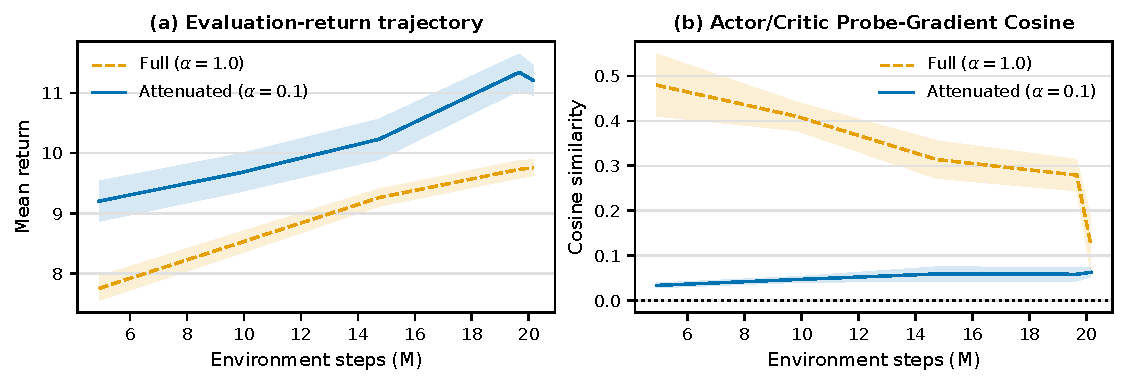
\includegraphics[width=0.88\textwidth]{plots/appendix/gradient_shielding_trajectories.pdf}
    \caption{\textbf{GGS checkpoint trajectories on Craftax-Classic.} Mean evaluation return and Actor/Critic Probe-Gradient Cosine for attenuated ($\alpha=0.1$) and full ($\alpha=1.0$) actor gradients. Shading is $\pm$ one standard error across the five matched runs at each checkpoint. The cosine uses diagnostic output sensitivities, not PPO actor- and critic-loss gradients.}
    \label{fig:app_ggs_trajectories}
\end{figure}

Figure~\ref{fig:app_ggs_trajectories} shows the training-time context for the endpoint-first main figure. The two return trajectories remain separated at the checkpoints, while the diagnostic cosine changes with gradient scale; neither repeated checkpoint is treated as an independent experimental unit.

\begin{figure}[htbp]
    \centering
    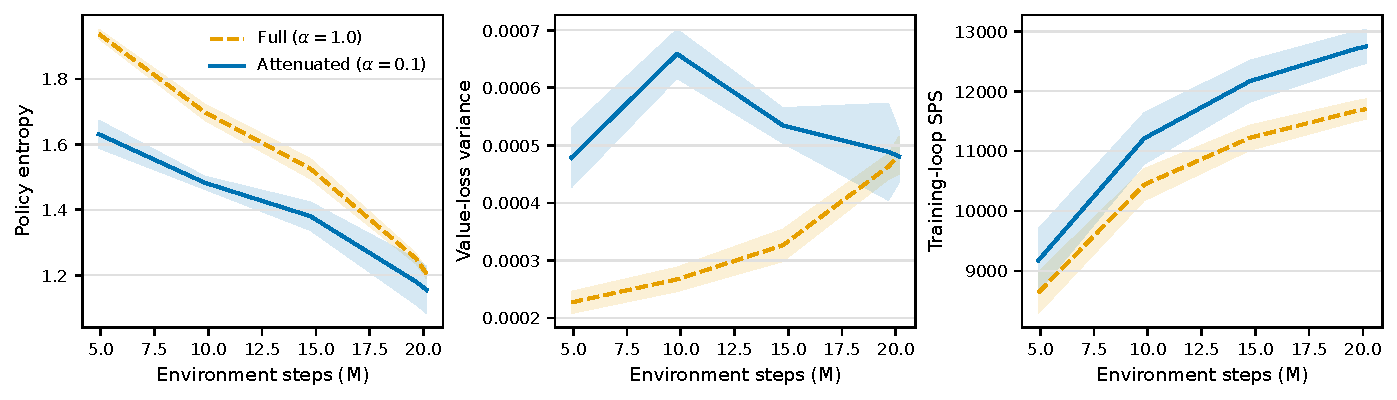
\includegraphics[width=0.95\textwidth]{plots/appendix/gradient_shielding_auxiliary.pdf}
    \caption{\textbf{Auxiliary GGS telemetry on Craftax-Classic.} Mean policy entropy, value-loss variance, and training-loop SPS trajectories for attenuated ($\alpha=0.1$) and full ($\alpha=1.0$) actor gradients. Shading is $\pm$ one standard error across five matched runs at each checkpoint.}
    \label{fig:app_ggs_auxiliary}
\end{figure}

Figure~\ref{fig:app_ggs_auxiliary} provides optimization telemetry complementary to the endpoint comparison. These trajectories are descriptive diagnostics from the same five-run GGS study; repeated checkpoints are not treated as independent experimental units.


%%%%%%%%%%%%%%%%%%%%%%%%%%%%%%%%%%%%%%%%%%%%%%%%%%%%%%%%%%%%%%%%%%%%%%%%%%%%%%%
% APPENDIX D: Experiment-by-Experiment Reproduction Protocol
%%%%%%%%%%%%%%%%%%%%%%%%%%%%%%%%%%%%%%%%%%%%%%%%%%%%%%%%%%%%%%%%%%%%%%%%%%%%%%%
\clearpage
\section{Experiment-by-Experiment Reproduction Protocol}
\label{app:experiment_protocols}

The entries below identify the executable family, protocol, and evidence for each reported result. Commands are collected in Appendix~\ref{app:repro_checklist}.

\subsection{Study-Specific SdLG Hyperparameters}
T-Maze uses $d_{\text{model}}=128$, three layers, $d_k=d_v=32$, $W=16$, an unfactorized Exact state, and an Approximate state with $r=16$ stored rows. In its NoRoPE condition, cosine symmetry leaves eight distinct row trajectories in exact arithmetic. MiniGrid uses the same width, depth, key, and value dimensions with $r=4$ and compares SWA enabled with bypassed. GGS uses $d_{\text{model}}=256$, four layers, $d_k=d_v=32$, $r=4$, and $W=8$. The study records provide the remaining optimizer, rollout, seed, and endpoint fields.

\subsection{Craftax-Classic Open-World Survival}
\begin{itemize}
    \item \textbf{Objective:} Evaluate macro-performance on a complex symbolic POMDP with dense crafting rewards and multi-step survival dynamics.
    \item \textbf{Operational Role:} Characterize architecture-dependent response to rollout/TBPTT length and record return--systems trade-offs across protocol-matched but capacity-unmatched families.
    \item \textbf{Configuration ID:} \texttt{T3-CRAFTAX-EXTERNAL-LANDSCAPE}. The repository's executable family is \path{scripts/diagnostics/benchmarks/craftax_full/craftax_classic_benchmark.py}.
    \item \textbf{Compared Models:} PPO-GTrXL, PPO-GRU, PPO-Mamba, PPO-GLA, AGaLiTe, SdLG-Approx (runner name \texttt{SdLGHybrid}), and SdLG-Exact in the five-run $T=64$ comparison.
    \item \textbf{Training Protocol:} 50M-step budgets and $T\in\{16,32,64,128\}$ for the cross-$T$ block; summaries use the final logged training return. The fixed-$T=64$ comparison has endpoint 49,971,200 and cumulative loop-SPS measurements.
    \item \textbf{Seed Coverage:} five runs at every reported cross-$T$ cell; see the explicit cell table below. The fixed-$T=64$ systems landscape uses seeds $42,43,44,45,46$.
    \item \textbf{Outputs:} Table~\ref{tab:app_craftax_returns} reports the training-return summaries. The SdLG-Approx W\&B runs use the final logged \texttt{Train/Mean\_Return}; metric sources are detailed in Appendix~\ref{app:craftax_cross_t_provenance}.
    \item \textbf{Main Paper Location:} Main text Section 5.5; additional Craftax results appear here. Reproduction commands are collected in Appendix~\ref{app:repro_checklist}.
\end{itemize}

\subsection{Passive T-Maze Cross-Family Baselines}
\label{app:tmaze_external_landscape}

This study compares eight recurrent configurations at training horizon $H=100$ and truncation length $T=16$ on seeds $\{101,102,103,104,123,456,789\}$. Every run has a 50M-step maximum budget and the same stopping rule: evaluate the terminal policy after three consecutive logged training returns reach $0.98$, or at the budget cap if the criterion is not reached. The configurations share a protocol but differ in capacity. Table~\ref{tab:tmaze_overview} places their terminal-policy returns beside the two SdLG studies without treating the separate seed sets as paired samples.

\begin{table}[H]
\centering\footnotesize
\setlength{\tabcolsep}{3.2pt}
\renewcommand{\arraystretch}{1.05}
\caption{\textbf{Passive T-Maze evaluation returns across studies.} Entries are mean $\pm$ sample SD over independent seeded runs. Row groups are separate studies with their own seed sets and configurations; comparisons across groups are descriptive rather than paired.}
\label{tab:tmaze_overview}
\begin{tabular}{lrrrr}
\toprule
Study / condition & $n$ & $H=100$ & $H=150$ & $H=200$ \\
\midrule
\multicolumn{5}{l}{\textit{Cross-family baselines}} \\
GRU              & 7  & $0.644\pm0.243$ & $0.426\pm0.345$ & $0.574\pm0.188$ \\
LSTM             & 7  & $0.571\pm0.189$ & $0.503\pm0.008$ & $0.433\pm0.191$ \\
Mamba            & 7  & $0.499\pm0.008$ & $0.499\pm0.008$ & $0.499\pm0.008$ \\
LTI-Linear       & 7  & $0.501\pm0.008$ & $0.501\pm0.008$ & $0.501\pm0.008$ \\
Markovian        & 7  & $0.506\pm0.006$ & $0.506\pm0.006$ & $0.506\pm0.006$ \\
GLA              & 7  & $0.782\pm0.271$ & $0.782\pm0.271$ & $0.710\pm0.271$ \\
GTrXL-64         & 7  & $0.930\pm0.186$ & $0.501\pm0.008$ & $0.501\pm0.008$ \\
GTrXL-128        & 7  & $1.000\pm0.000$ & $0.574\pm0.188$ & $0.503\pm0.008$ \\
\midrule
\multicolumn{5}{l}{\textit{SdLG execution $\times$ phase factorial}} \\
Exact-NoRoPE     & 10 & $0.900\pm0.211$ & $0.900\pm0.211$ & $0.851\pm0.240$ \\
Exact-RoPE       & 10 & $0.800\pm0.258$ & $0.602\pm0.210$ & $0.651\pm0.241$ \\
Approx-NoRoPE    & 10 & $0.498\pm0.008$ & $0.548\pm0.159$ & $0.498\pm0.008$ \\
Approx-RoPE      & 10 & $0.651\pm0.241$ & $0.503\pm0.008$ & $0.502\pm0.008$ \\
\midrule
\multicolumn{5}{l}{\textit{Matched SdLG formulation control}} \\
Matched Exact    & 10 & $0.900\pm0.211$ & $0.900\pm0.211$ & $0.851\pm0.240$ \\
Matched Approx.  & 10 & $0.398\pm0.210$ & $0.502\pm0.008$ & $0.500\pm0.008$ \\
\bottomrule
\end{tabular}
\end{table}

Main Table~\ref{tab:tmaze_external_main} reports the baseline parameter counts, stopping outcomes, and terminal steps. The two GTrXL rows differ in memory length but not trainable parameters. The $H=250$ fields are excluded because the environment's 200-step limit terminates evaluation before the delayed decision. Runs labelled ``S5'' are excluded because they use $T=64$ and implement the same simplified diagonal recurrence represented here as LTI-Linear.

\subsection{Passive T-Maze Factorial Horizon Evaluation \texorpdfstring{($H=100,150,200$)}{(H=100,150,200)}}
\begin{itemize}
    \item \textbf{Objective:} Characterize long-horizon state execution and positional-phase behavior under severe gradient truncation ($T=16$).
    \item \textbf{Operational Question:} How do state execution and positional phase change trained- and unseen-horizon behavior when $H\gg T$? The boundary statistic tests for a localized shift in squared value-target error; it does not measure representation drift or bootstrap corruption directly.
    \item \textbf{Configuration ID:} \texttt{T1-TMAZE-EXECUTION-PHASE} \\ ($\to$ \path{scripts/diagnostics/exact_sdlg/exact_sdlg_tmaze_ablations.py}).
    \item \textbf{Compared Variants:} \texttt{Exact\_NoRoPE}, \texttt{Exact\_RoPE} (unfactorized full-matrix state), \texttt{Approx\_RoPE}, and \texttt{Approx\_NoRoPE} (Approximate with $r=16$ stored rows; the NoRoPE cosine construction has eight duplicated row pairs).
    \item \textbf{Training Protocol:} $d_{\text{model}}=128$, three layers, $d_k=d_v=32$, $W=16$, $N_{\text{envs}}=1024$, $H_{\text{train}}=100$, $T=16$, 50M-step cap, and early stopping after three consecutive logged training returns reach $0.98$; learning rate $5\times 10^{-4}$ with 4 PPO epochs / 8 minibatches.
    \item \textbf{Evaluation Protocol \& Horizon:} In-domain evaluation at $H_{\text{train}}=100$ and zero-shot extrapolation to $H \in \{100, 150, 200\}$.
    \item \textbf{Seeds:} 10 random seeds ($42, 54, 99, 123, 456, 789, 111, 222, 333, 444$).
    \item \textbf{Solving Rates:} A seed is classified as solved when its terminal deterministic evaluation success proportion across 256 episodes is at least $0.90$; this differs from the training stopping rule. At $H=100$ and $H=200$, respectively, the rates are $80.0\%$ and $70.0\%$ for \texttt{Exact\_NoRoPE}, $60.0\%$ and $30.0\%$ for \texttt{Exact\_RoPE}, $30.0\%$ and $0.0\%$ for \texttt{Approx\_RoPE}, and $0.0\%$ at both horizons for \texttt{Approx\_NoRoPE}.
    \item \textbf{Evidence:} Seed-level terminal-step and horizon-return records underlie the means and sample SDs in Table~\ref{tab:tmaze_overview}.
    \item \textbf{Main Paper Location:} Main text Section 5.1 and Figure 2.
    \item \textbf{Reproduction:} Commands are collected in Appendix~\ref{app:repro_checklist}.
\end{itemize}

\paragraph{Factorial contrast.}
The four cells are analyzed as independent seed-level samples; matching integer labels alone is not treated as verified trajectory pairing. Figure~\ref{fig:tmaze_factorial}c reports the $H=200$ difference between the mean of the two Exact cells and the mean of the two Approximate cells, with a percentile-bootstrap 95\% interval from 200,000 independent-cell resamples.

Early-stopping time does not track unseen-horizon return monotonically in the factorial. The boundary diagnostic gives a boundary-minus-interior squared value-target-error statistic of approximately $-0.011$ for both execution families, so it does not reveal a boundary-local increase in that measured quantity. This statistic is not TD-error variance, a representation-drift measure, or a general test of bootstrap correctness.

\subsection{Topology- and Gradient-Matched T-Maze Execution}
\label{app:tmaze_matched_execution}
The matched configuration ID \texttt{T1-TMAZE-MATCHED-EXECUTION} holds fixed three local--associative--gated-FFN blocks, $d_{\mathrm{model}}=128$, $d_k=d_v=32$, $W=16$, NoRoPE, and an unattenuated common actor--critic trunk ($\alpha=1$). It compares the full-matrix Exact and factorized Approximate state-execution paths, with $r=16$ stored rows; under NoRoPE, cosine symmetry makes these eight pairs of duplicated trajectories in exact arithmetic. The ten runs per condition are analyzed as independent seed-level samples. Two short seed-42 validation runs are excluded; for seed 222, the completed Approximate run is used in place of an interrupted attempt. At $H=200$, Exact reaches $0.851\pm0.240$ and Approximate $0.500\pm0.008$; the independent-condition difference is $0.351\,[0.200,0.497]$.

Matched Exact has nine successful early stops and one 50M-step-censored run (mean terminal step 9.08M); Matched Approximate has seven successful early stops and three censored runs (mean terminal step 26.18M). These training-time outcomes remain separate from the horizon-return analysis. It remains a formulation-level comparison: full-matrix versus factorized state, recurrence/update, normalized read, effective state size, and numerical path still change jointly, so it does not isolate rank alone.

\paragraph{Comparability with the original factorial.}
The matched control was designed after the original factorial and used NoRoPE, its best-performing Exact phase setting; the phase choice was therefore not prospectively independent of the factorial results. Original-factorial Exact-NoRoPE and Matched Exact have identical means and sample SDs at all three horizons, but their seed-labelled endpoints differ for 4/10, 4/10, and 6/10 seeds at $H=100,150,200$, respectively. At $H=200$, for example, seed 54 changes from $1.000$ to $0.508$, while seed 123 changes from $0.508$ to $1.000$. Aggregate equality therefore establishes neither reused seed-level outcomes nor independent replication.

\begin{table}[H]
\centering\small
\begin{tabularx}{\linewidth}{l>{\centering\arraybackslash}X>{\centering\arraybackslash}Xc}
\toprule
Study & Exact & Approx. & Fisher $p$ \\
\midrule
Original factorial & 7/10 $[0.397,0.892]$ & 0/10 $[0.000,0.278]$ & $0.00310$ \\
Matched control & 7/10 $[0.397,0.892]$ & 0/10 $[0.000,0.278]$ & $0.00310$ \\
\bottomrule
\end{tabularx}

\caption{\textbf{Exploratory T-Maze solve summaries at $H=200$.} A seed is solved when its terminal deterministic evaluation success proportion is at least $0.90$. Brackets are Wilson 95\% intervals for each proportion; Fisher tests are two-sided independent-condition comparisons. These post hoc threshold analyses are pointwise, unadjusted, and supplementary to the primary continuous-return contrasts.}
\label{tab:tmaze_solve_exploratory}
\end{table}

Both studies yield the same aggregate solve table, although their Exact seed-level outcomes differ as described above; Table~\ref{tab:tmaze_solve_exploratory} reports the resulting solve counts and intervals.

\subsection{MiniGrid Spatial Retention \& SWA Ablation}
\begin{itemize}
    \item \textbf{Objective:} Test whether enabling localized Sliding Window Attention (SWA) changes performance on XLand-MiniGrid MemoryS16~\cite{minigrid,nikulin2024xland}.
    \item \textbf{Operational Question:} Does SWA-enabled execution differ from SWA-bypassed execution? Task return does not identify a unique cue-storage or interference mechanism.
    \item \textbf{Observation Space:} $3 \times 3 \times 2$ egocentric grid ($18$ flattened symbolic features) in \texttt{xminigrid}.
    \item \textbf{Parameter Control:} Both conditions share $d_{\text{model}}=128$, three layers, four heads, $d_k=d_v=32$, rank 4, FFN 512, and \texttt{WINDOW\_SIZE=16}; bypass uses \texttt{local\_mode="none"}.
    \item \textbf{Configuration ID:} \texttt{T1-MINIGRID-LOCAL-WINDOW} \\ ($\to$ \path{scripts/diagnostics/architecture/swa_ablation/swa_ablation.py}).
    \item \textbf{Compared Models:} SdLG-Approx with SWA enabled versus SWA bypassed.
    \item \textbf{Training Protocol:} 10M-step target, fixed logged endpoint 9,830,400, $N_{\text{envs}}=256$, $T=64$, learning rate $3\times 10^{-4}$, 4 PPO epochs / 8 minibatches.
    \item \textbf{Evaluation Protocol \& Horizon:} final \texttt{Eval/Mean\_Return} at the common logged endpoint.
    \item \textbf{Seeds:} 15 independent runs per condition ($42,54,99,123,456,111,222,333,444,789,1001,1002,1003,1004,1005$).
    \item \textbf{Source Control:} All 30 reported runs use the same code and environment configuration.
    \item \textbf{Primary Quantitative Output:} SWA-enabled mean return $0.508$ (SD $0.445$) versus bypassed mean $0.782$ (SD $0.354$); the independent-bootstrap interval for enabled minus bypassed is $[-0.549,0.008]$.
    \item \textbf{Paper Location:} Main text Section~\ref{sec:optional_controls}; full seed-level display below.
    \item \textbf{Reproduction:} The fixed-endpoint command is given in Appendix~\ref{app:repro_checklist}.
\end{itemize}

\begin{figure}[htbp]
\centering
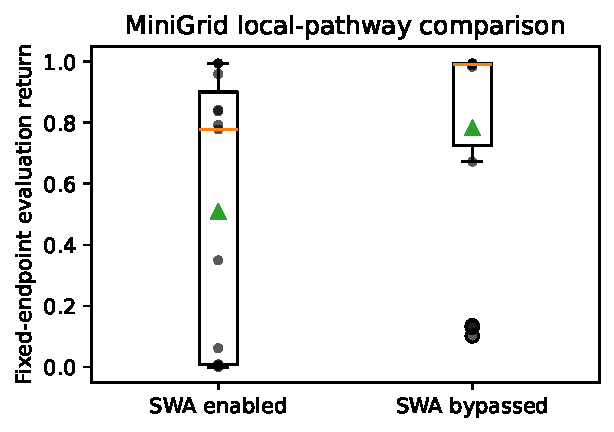
\includegraphics[width=0.62\textwidth]{plots/rebuilt/fig5_minigrid_locality_expanded.pdf}
\caption{\textbf{MiniGrid local-pathway comparison.} Fixed-endpoint returns for 15 independent runs per condition. Diamonds and bars show means with condition-level 95\% bootstrap intervals.}
\label{fig:minigrid_ablation}
\end{figure}

\subsection{DoorKey-8x8 Cross-Family Study: Five Seeds}
\label{app:doorkey_8x8}

The study compares SdLG-Exact, PPO-GRU, and PPO-GTrXL on seeds $\{42,54,99,123,456\}$. Table~\ref{tab:doorkey_8x8_summary} reports arithmetic means and sample SDs (denominator $n-1$) across all five runs per model; no failed-learning run is excluded. E/C denotes early-stop versus cap outcomes. Parameter counts are instantiated trainable totals, not matched budgets.

\begin{table}[H]
\centering\footnotesize
\setlength{\tabcolsep}{3.5pt}
\caption{\textbf{DoorKey-8x8 terminal-policy results.} Five seeds per model; mean $\pm$ sample SD across runs. Success rates are fractions, not percentages.}
\label{tab:doorkey_8x8_summary}
\begin{tabular}{lrrrrr}
\toprule
Model & Parameters & Runs & E/C & Eval. return & Success rate \\
\midrule
SdLG-Exact & 1,634,983 & 5/5 & 3/2 & $0.668\pm0.408$ & $0.748\pm0.362$ \\
PPO-GRU & 326,791 & 5/5 & 1/4 & $0.193\pm0.432$ & $0.200\pm0.447$ \\
PPO-GTrXL & 969,479 & 5/5 & 2/3 & $0.468\pm0.466$ & $0.537\pm0.446$ \\
\bottomrule
\end{tabular}

\end{table}

\paragraph{Training and evaluation protocol.}
The shared encoder divides the $7\times7\times2$ symbolic observation by ten, flattens it, and applies two width-128 ReLU layers followed by layer normalization. Each core uses three layers at width 128; Exact uses four heads with $d_k=d_v=32$, feed-forward width 512, local window 16, and NoRoPE; GTrXL uses four heads of width 32 and memory length 128. The common actor and critic heads operate on each core's output. Table~\ref{tab:doorkey_8x8_protocol} records the shared optimization settings.

\begin{table}[H]
\centering\small
\caption{\textbf{DoorKey-8x8 protocol.} This experiment differs from the MemoryS16 SWA intervention.}
\label{tab:doorkey_8x8_protocol}
\begin{tabular}{ll}
\toprule
Setting & Value \\
\midrule
Parallel environments / rollout length & $512$ / $64$ \\
PPO epochs / minibatches & $4$ / $8$ \\
Learning rate / schedule & $3\times10^{-4}$ / linear annealing \\
Discount / GAE $\lambda$ & $0.99$ / $0.95$ \\
PPO clip / entropy / value coefficients & $0.2$ / $0.01$ / $0.5$ \\
Gradient norm cap / Adam $\epsilon$ & $0.5$ / $10^{-5}$ \\
Logging interval & $10$ updates ($327{,}680$ environment steps) \\
Stopping rule & Training mean return $\geq0.96$ for $3$ consecutive intervals \\
Target cap / last complete block & $20{,}000{,}000$ / $19{,}988{,}480$ steps \\
Terminal evaluation & $256$ stochastic-policy episodes; maximum length $640$ \\
Evaluation PRNG seed & $100{,}000+s$ for training seed $s$ \\
\bottomrule
\end{tabular}
\end{table}

Evaluation accumulates each environment's first episode only, samples categorical actions, and defines success as positive episode return. All 15 terminal evaluations have completion rate $1.0$, and model groups are summarized independently.

\begin{table}[H]
\centering\footnotesize
\setlength{\tabcolsep}{4pt}
\caption{\textbf{DoorKey-8x8 run-level results.} Every row corresponds to one terminal evaluation. Steps are rounded to five decimal places in millions.}
\label{tab:doorkey_8x8_runs}
\begin{tabular}{lrrlrrl}
\toprule
Model & Seed & Steps (M) & Stop & Eval. return & Success & Offline run ID \\
\midrule
SdLG-Exact & 42 & 10.15808 & early & 0.946671 & 0.992188 & \texttt{rw1bumxt} \\
SdLG-Exact & 54 & 19.98848 & cap & 0.338656 & 0.542969 & \texttt{e4hlu9rj} \\
SdLG-Exact & 99 & 10.81344 & early & 0.968848 & 1.000000 & \texttt{5gt0fm5f} \\
SdLG-Exact & 123 & 12.77952 & early & 0.967437 & 1.000000 & \texttt{qnk6ianb} \\
SdLG-Exact & 456 & 19.98848 & cap & 0.120354 & 0.203125 & \texttt{nbbct6nk} \\
PPO-GRU & 42 & 18.02240 & early & 0.966739 & 1.000000 & \texttt{ngzqqmkb} \\
PPO-GRU & 54 & 19.98848 & cap & 0.000000 & 0.000000 & \texttt{ge8rfkxu} \\
PPO-GRU & 99 & 19.98848 & cap & 0.000000 & 0.000000 & \texttt{1geyiyfm} \\
PPO-GRU & 123 & 19.98848 & cap & 0.000000 & 0.000000 & \texttt{1hftr7qx} \\
PPO-GRU & 456 & 19.98848 & cap & 0.000000 & 0.000000 & \texttt{sybbpvm2} \\
PPO-GTrXL & 42 & 19.98848 & cap & 0.034774 & 0.050781 & \texttt{uws921pn} \\
PPO-GTrXL & 54 & 19.98848 & cap & 0.099736 & 0.187500 & \texttt{ney2o0n3} \\
PPO-GTrXL & 99 & 7.53664 & early & 0.968376 & 1.000000 & \texttt{m6ld3lo4} \\
PPO-GTrXL & 123 & 19.98848 & cap & 0.267422 & 0.445312 & \texttt{cqoswapp} \\
PPO-GTrXL & 456 & 7.53664 & early & 0.971891 & 1.000000 & \texttt{ybtvect1} \\
\bottomrule
\end{tabular}

\end{table}

\paragraph{Reproduction record.}
Tables~\ref{tab:doorkey_8x8_summary} and~\ref{tab:doorkey_8x8_runs} report the aggregate and run-level DoorKey results. All 15 runs follow the stated 8x8 protocol, with one terminal record per model--seed cell; interrupted attempts are not additional samples. The runs used Python 3.12.3 with JAX/JAXlib 0.6.0, Flax 0.10.7, Optax 0.2.8, and XMiniGrid 0.9.3 on the Radeon RX 6800 XT workstation. Commands are collected in Appendix~\ref{app:repro_checklist}.

\subsection{POPGym Benchmark Suite \& Capacity Probes}
\begin{itemize}
    \item \textbf{Objective:} Report operation-specific behavior across 16 Easy and 7 Medium partially observable tasks, including card matching and continuous tracking.
    \item \textbf{Interpretive Scope:} Model families differ in parameter count, architecture, and optimization, so results are reported per task rather than pooled.
    \item \textbf{Configuration ID:} \texttt{T3-POPGYM-SUITE}; task, model, seed, and endpoint records cover 16 Easy and 7 Medium tasks. A complete mapping from the available run records to source revisions and configurations is not available for every task--model cell.
    \item \textbf{Compared Models:} The project evaluations cover SdLG-Exact, SdLG-Approx, PPO-GRU, PPO-Mamba, and PPO-GLA, with models varying by task. \citet{morad2023popgym} report 13 memory-model baselines in their Table~3; Appendix Tables~\ref{table:popgym_published_easy_1}--\ref{table:popgym_published_medium_2} reproduce the overlapping source rows as external context without pooling them with the project trials.
    \item \textbf{Protocol Status:} The examples use seeds $\{42,43,44\}$. Concentration runs reach 14,909,440 steps, while one CountRecall run ends at 14,581,760; these MMER examples are not a common fixed-endpoint block. The full suite uses each cell's seed coverage and endpoint semantics.
    \item \textbf{Evaluation Semantics:} Task-native Max-Mean Episodic Reward (MMER): for each seed, the maximum logged \texttt{Eval\_Return\_H100}, followed by mean and sample SD across its seeds.
    \item \textbf{Primary Quantitative Output:} Task-native MMER values and seed coverage, including contrasting orderings on \texttt{CountRecallEasy}, \texttt{ConcentrationEasy}, and \texttt{RepeatFirstEasy}.
    \item \textbf{Main Paper Location:} Section~\ref{sec:popgym_results} summarizes the task comparisons; Appendix E contains the examples and complete tables.
    \item \textbf{Reproduction:} The one-cell implementation check is given in Appendix~\ref{app:repro_checklist}.
\end{itemize}

\subsection{GGS Actor-Critic Gradient Shielding Ablation}
\begin{itemize}
    \item \textbf{Objective:} Evaluate whether modulating the actor gradient entering shared sequence layers through Gradient Gating Scale ($\alpha \in [0.0, 1.0]$) changes optimization trajectories and endpoint return.
    \item \textbf{Operational Question:} Do $\alpha=0.1$ and $\alpha=1.0$ produce different return and probe-gradient telemetry under a shared protocol? The probe does not test causal mediation or representation corruption.
    \item \textbf{Configuration ID:} \texttt{T1-CRAFTAX-ACTOR-GRADIENT-SCALE} \\ ($\to$ \path{scripts/diagnostics/architecture/gradient_shielding/gradient_shielding.py}).
    \item \textbf{Compared Models:} \texttt{SdLG-GGS-0.1} (attenuated actor gradient) vs. \texttt{SdLG-GGS-1.0} (full actor gradient).
    \item \textbf{Training Protocol:} 20M-step target, $N_{\text{envs}}=256$, $T=64$, $d_{\text{model}}=256$, four layers, eight heads, $d_k=d_v=32$, rank 4, $W=8$, learning rate $3\times 10^{-4}$.
    \item \textbf{Evaluation Protocol \& Horizon:} Final evaluation at 20,152,320 environment steps; return and probe telemetry are aggregated across five seeded runs.
    \item \textbf{Seeds and Pairing:} five matched seeds ($42,54,99,123,456$). Both conditions receive the same seed-specific PRNG key, initialization, random-number streams, and fixed evaluation seeds; only $\alpha$ changes. This provides a matched common-random-numbers design, although realized trajectories may diverge as the policies diverge. Endpoint uncertainty therefore uses paired resampling of seeded runs.
    \item \textbf{Endpoint Returns by Seed:} for $\alpha=0.1$, $(10.483,11.484,11.198,11.956,10.927)$; for $\alpha=1.0$, $(9.903,9.614,10.184,9.684,9.400)$, in the seed order above (three decimals).
    \item \textbf{Primary Quantitative Output:} Mean endpoint return $11.210$ (SD $0.557$) for $\alpha=0.1$ and $9.757$ (SD $0.299$) for $\alpha=1.0$. The mean paired difference is $1.453$. The exhaustive paired percentile-bootstrap 95\% CI, $[0.925,1.962]$, excludes zero, while the exact two-sided paired sign-flip test gives $p=0.0625$; with only five pairs, we treat both as descriptive uncertainty summaries rather than a binary significance decision.
    \item \textbf{Excluded exploratory cell:} The reported comparison is restricted to $\alpha\in\{0.1,1.0\}$; one exploratory $\alpha=0$ run is excluded and is not used for a response-curve claim.
    \item \textbf{Main Paper Location:} Main text Section~\ref{sec:optional_controls} and Figure~\ref{fig:ggs_telemetry}; auxiliary telemetry remains in Appendix C.
    \item \textbf{Reproduction:} The training command is given in Appendix~\ref{app:repro_checklist}.
\end{itemize}

\subsection{Craftax Cross-$T$ Scope}
\label{app:craftax_cross_t_provenance}
\begin{itemize}
    \item \textbf{Configurations:} \texttt{SdLGHybrid} denotes the factorized SdLG-Approx implementation with $\widetilde K,\widetilde V$ state and a coupled actor--critic trunk. SdLG-Exact uses a full-matrix wrapper.
    \item \textbf{Metric separation:} The cross-$T$ table reports final logged training-episode return, not a validation or evaluation rollout. Each cell averages five endpoint values with sample SD after a 50M-step budget. These values are not combined with the $T=64$ loop-SPS comparison or the 20.15M-step GGS intervention.
    \item \textbf{Run cells:} Table~\ref{tab:app_craftax_returns} lists every family/$T$ cell that was run; missing cells are not imputed.
    \item \textbf{Reproduction:} The executable family and analysis-only verification are given in Appendix~\ref{app:repro_checklist}.
\end{itemize}

%%%%%%%%%%%%%%%%%%%%%%%%%%%%%%%%%%%%%%%%%%%%%%%%%%%%%%%%%%%%%%%%%%%%%%%%%%%%%%%
% APPENDIX E: Complete Benchmark Tables & Extended Telemetry
%%%%%%%%%%%%%%%%%%%%%%%%%%%%%%%%%%%%%%%%%%%%%%%%%%%%%%%%%%%%%%%%%%%%%%%%%%%%%%%
\section{Complete Benchmark Tables \& Extended Telemetry}
\label{app:full_results}

This section provides diagnostic telemetry figures, structural ablation tables, and the project result tables for the POPGym suite. It also reproduces the relevant rows from the original benchmark's 13-model MMER reference table~\citep{morad2023popgym}. Project and published trials are reported in different tables because their implementations, endpoints, and seed coverage do not form one controlled comparison.

\subsection{Craftax External Landscape and Systems Scope}
\begin{table}[htbp]
\centering\small
\setlength{\tabcolsep}{3.5pt}
\caption{\textbf{Craftax final logged training-return summaries.} Each reported cell is a mean $\pm$ sample SD across five runs after a 50M-step target. The first five families form the fixed-$T=64$ systems comparison; the two SdLG rows come from the cross-$T$ experiment described in Appendix~\ref{app:craftax_cross_t_provenance}. Parameter counts provide context rather than capacity matching. Dashes denote cells that were not run.}
\label{tab:app_craftax_returns}
\begin{tabular}{lrrrrr}
\toprule
Family & Parameters & $T=16$ & $T=32$ & $T=64$ & $T=128$ \\
\midrule
PPO-GLA   & 6,810,130 & $14.11\pm0.59$ & -- & $15.69\pm0.22$ & -- \\
PPO-GRU   &   809,234 & $16.44\pm0.11$ & -- & $15.59\pm0.30$ & $15.62\pm0.11$ \\
PPO-GTrXL & 5,409,554 & -- & -- & $15.40\pm0.22$ & $13.83\pm0.68$ \\
AGaLiTe   & 7,338,610 & $14.44\pm0.61$ & $14.99\pm0.26$ & $15.12\pm0.20$ & -- \\
PPO-Mamba &   850,194 & $15.86\pm0.07$ & -- & $14.97\pm0.33$ & -- \\
\midrule
SdLG-Approx & 6,110,000 & $16.33\pm0.37$ & -- & $14.79\pm0.36$ & -- \\
SdLG-Exact  & 8,780,000 & -- & -- & $13.70\pm0.52$ & -- \\
\bottomrule
\end{tabular}
\end{table}

\begin{figure}[htbp]
\centering
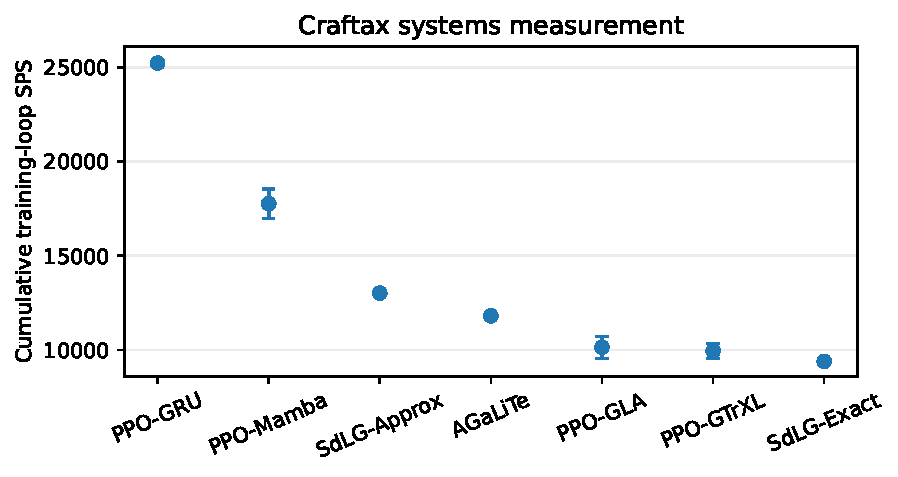
\includegraphics[width=0.82\textwidth]{plots/rebuilt/fig4_craftax_throughput.pdf}
\caption{\textbf{Craftax systems scope.} Cumulative training-loop SPS for the evaluated procedures; whiskers show seed SD where estimated. The measurement includes compilation, warm-up, environment interaction, optimization, and logging; it is not an inference-latency or kernel-only benchmark.}
\label{fig:app_craftax_throughput}
\end{figure}

Figure~\ref{fig:app_craftax_throughput} shows the end-to-end loop measurement: PPO-GRU has the highest mean SPS among these seven procedures. Because the measurement includes compilation, warm-up, environment interaction, optimization, and logging, it is not interpreted as recurrent-kernel or inference latency.

\subsection{Minesweeper Recurrent Depth vs. Rank Scale Ablation}
\label{app:minesweeper_ablation}
This three-seed comparison changes layer order, recurrent depth, and rank jointly. The duplicated $H=100$ and $H=200$ source values do not support extrapolation; Table~\ref{table:minesweeper_ablation_summary} provides structural scope only.

\begin{table}[htbp]
\caption{\textbf{Minesweeper Structural Ablation Study ($15\text{M}$ steps, $T=64$).} Evaluation normalized scores at $H=100$ and $H=200$, plus execution throughput (SPS). The identical source values provide structural scope rather than length-extrapolation evidence.}
\label{table:minesweeper_ablation_summary}
\vskip 0.1in
\begin{center}
\begin{small}
\resizebox{\textwidth}{!}{%
\begin{tabular}{l c c c c}
\toprule
\textbf{Architecture Variant} & \textbf{Structural Parameter} & \textbf{Eval Score ($H=100$)} & \textbf{Eval Score ($H=200$)} & \textbf{Throughput (SPS)} \\
\midrule
\textbf{SdLG-1GLA-r16} & Single Layer, Rank Scale ($r=16$) & $0.445 \pm 0.031$ & $0.445 \pm 0.031$ & \textbf{1,698.8} \\
\textbf{SdLG-2GLA-r4} & Dual Layer, Recurrent Depth ($r=4$) & \textbf{0.549 $\pm$ 0.024} & \textbf{0.549 $\pm$ 0.024} & 1,617.9 \\
\textbf{SdLG-3GLA-r4} & Triple Layer, Homogeneous Depth ($r=4$) & $0.527 \pm 0.028$ & $0.527 \pm 0.028$ & 1,488.7 \\
\bottomrule
\end{tabular}
}
\end{small}
\end{center}
\end{table}

\clearpage
\begin{table}[H]
\centering\small
\setlength{\tabcolsep}{3pt}
\renewcommand{\arraystretch}{1.12}
\caption{\textbf{POPGym Easy Suite: evaluated models.} Project MMER ($\mu\pm\sigma$ across reported seeds), with $d_{\mathrm{model}}=128$. Model capacities are unmatched. Published POPGym reference trials appear in Tables~\ref{table:popgym_published_easy_1} and~\ref{table:popgym_published_easy_2}.}
\label{table:popgym_easy_full}
\begin{tabular}{@{}p{0.30\textwidth}ccccc@{}}
\toprule
Environment & SdLG-Exact & SdLG-Approx & PPO-GRU & PPO-Mamba & PPO-GLA \\
\midrule
AutoencodeEasy & $-0.351 \pm 0.017$ & $-0.333 \pm 0.066$ & $-0.270 \pm 0.007$ & $-0.368 \pm 0.021$ & $-0.339 \pm 0.022$ \\
BattleshipEasy & $-0.505 \pm 0.024$ & $-0.684 \pm 0.150$ & $-0.400 \pm 0.024$ & $-0.253 \pm 0.048$ & $0.026 \pm 0.036$ \\
ConcentrationEasy & $-0.267 \pm 0.011$ & $-0.102 \pm 0.007$ & $0.158 \pm 0.026$ & $-0.359 \pm 0.030$ & $-0.099 \pm 0.100$ \\
CountRecallEasy & $0.670 \pm 0.113$ & $-0.712 \pm 0.013$ & $-0.048 \pm 0.043$ & $-0.292 \pm 0.075$ & $0.062 \pm 0.062$ \\
HigherLowerEasy & $0.539 \pm 0.004$ & $0.535 \pm 0.005$ & $0.548 \pm 0.006$ & $0.544 \pm 0.009$ & $0.561 \pm 0.011$ \\
LabyrinthEscapeEasy & $0.671 \pm 0.054$ & $0.967 \pm 0.002$ & $0.971 \pm 0.002$ & $0.970 \pm 0.001$ & $0.746 \pm 0.387$ \\
LabyrinthExploreEasy & $0.946 \pm 0.009$ & $0.965 \pm 0.009$ & $0.972 \pm 0.002$ & $0.973 \pm 0.001$ & $0.968 \pm 0.003$ \\
MinesweeperEasy & $0.591 \pm 0.090$ & $0.594 \pm 0.082$ & $0.942 \pm 0.011$ & $0.946 \pm 0.035$ & $0.938 \pm 0.054$ \\
MultiarmedBanditEasy & $0.616 \pm 0.011$ & $0.467 \pm 0.038$ & $0.640 \pm 0.045$ & $0.634 \pm 0.032$ & -- \\
NoisyPositionOnly\allowbreak{}CartPoleEasy & $0.432^\dagger$ & $0.421^\dagger$ & -- & -- & -- \\
NoisyPositionOnly\allowbreak{}PendulumEasy & $0.716^\dagger$ & $0.588^\dagger$ & -- & -- & -- \\
PositionOnlyCartPoleEasy & $1.000 \pm 0.000$ & $0.998 \pm 0.006$ & $1.000 \pm 0.000$ & $1.000 \pm 0.000$ & $1.000 \pm 0.000$ \\
PositionOnly\allowbreak{}PendulumEasy & $0.792^\dagger$ & $0.671^\dagger$ & -- & -- & -- \\
RepeatFirstEasy & $0.999 \pm 0.002$ & $0.619 \pm 0.127$ & $1.000 \pm 0.000$ & $0.073 \pm 0.023$ & $1.000 \pm 0.000$ \\
RepeatPreviousEasy & $0.741 \pm 0.352$ & $0.536 \pm 0.255$ & $0.963 \pm 0.014$ & $0.864 \pm 0.079$ & $0.823 \pm 0.123$ \\
VelocityOnlyCartpoleEasy & $1.000^\dagger$ & $1.000^\dagger$ & -- & -- & -- \\
\bottomrule
\end{tabular}
\par\smallskip\raggedright
\textit{Note:} $\dagger$ denotes a single-seed cell ($n=1$), reported without a standard deviation. Dashes denote unavailable cells.
\end{table}

\begin{table}[H]
\centering\small
\setlength{\tabcolsep}{3pt}
\renewcommand{\arraystretch}{1.12}
\caption{\textbf{POPGym Medium Suite: evaluated models.} Project MMER ($\mu\pm\sigma$ across reported seeds), with $d_{\mathrm{model}}=128$. Model capacities are unmatched. Published POPGym reference trials appear in Tables~\ref{table:popgym_published_medium_1} and~\ref{table:popgym_published_medium_2}.}
\label{table:popgym_medium_full}
\begin{tabular}{@{}p{0.30\textwidth}ccccc@{}}
\toprule
Environment & SdLG-Exact & SdLG-Approx & PPO-GRU & PPO-Mamba & PPO-GLA \\
\midrule
ConcentrationMedium & $-0.059 \pm 0.051$ & $0.007 \pm 0.004$ & $0.070 \pm 0.001$ & $-0.218 \pm 0.035$ & $-0.083 \pm 0.021$ \\
CountRecallMedium$^\dagger$ & $-0.800^\dagger$ & $-0.862^\dagger$ & $-0.538^\dagger$ & $-0.817^\dagger$ & $-0.763^\dagger$ \\
HigherLowerMedium$^\dagger$ & $0.516^\dagger$ & $0.509^\dagger$ & $0.510^\dagger$ & $0.511^\dagger$ & $0.511^\dagger$ \\
LabyrinthEscapeMedium & $-0.899 \pm 0.067$ & $-0.937 \pm 0.001$ & $-0.937 \pm 0.000$ & $-0.958 \pm 0.036$ & $-0.937 \pm 0.000$ \\
LabyrinthExploreMedium$^\dagger$ & $0.904^\dagger$ & $0.886^\dagger$ & $0.931^\dagger$ & $0.932^\dagger$ & $0.927^\dagger$ \\
MinesweeperMedium$^\dagger$ & $-0.246^\dagger$ & $-0.142^\dagger$ & $-0.039^\dagger$ & $0.206^\dagger$ & $0.234^\dagger$ \\
RepeatPreviousMedium & $-0.383 \pm 0.015$ & $-0.428 \pm 0.030$ & $-0.380 \pm 0.018$ & $-0.405 \pm 0.020$ & $-0.340 \pm 0.007$ \\
\bottomrule
\end{tabular}
\par\smallskip\raggedright
\textit{Note:} $\dagger$ denotes a single-seed cell ($n=1$), reported without a standard deviation. Dashes denote unavailable cells.
Unmarked cells have three seeds, except for PPO-GRU and PPO-Mamba on RepeatPreviousMedium, which have seven seeds each; daggered cells contain one seed.
\end{table}

\subsection{Published POPGym Reference Results}
Tables~\ref{table:popgym_published_easy_1}--\ref{table:popgym_published_medium_2} reproduce the POPGym benchmark results reported in Table~3 of \citet{morad2023popgym}. They include DNC, Elman, FART, FWP, Frame Stack, GRU, IndRNN, LMU, LSTM, MLP, PosMLP, S4D, and TCN. The source's \texttt{Stateless} task names correspond to the \texttt{PositionOnly} aliases used in this project. These published values contextualize score scale and task difficulty; they are not results from this project's runs and are not pooled with them.

\begin{table*}[p]
\centering\scriptsize
\setlength{\tabcolsep}{2.7pt}
\renewcommand{\arraystretch}{1.08}
\caption{\textbf{Published POPGym Easy reference (1/2).} MMER mean $\pm$ SD transcribed from Table~3 of \citet{morad2023popgym}. These source trials are external context and are not pooled with the project evaluations.}
\label{table:popgym_published_easy_1}
\begin{tabular}{@{}p{0.245\textwidth}ccccccc@{}}
\toprule
Project task & DNC & Elman & FART & FWP & Frame Stack & GRU & IndRNN \\
\midrule
AutoencodeEasy & $-.489\pm.002$ & $-.306\pm.022$ & $-.447\pm.014$ & $-.322\pm.020$ & $-.422\pm.010$ & $-.283\pm.029$ & $-.334\pm.004$ \\
BattleshipEasy & $-.427\pm.002$ & $-.290\pm.013$ & $-.413\pm.005$ & $-.389\pm.007$ & $-.378\pm.015$ & $-.320\pm.013$ & $-.287\pm.005$ \\
ConcentrationEasy & $-.182\pm.004$ & $-.098\pm.012$ & $-.185\pm.002$ & $-.188\pm.001$ & $-.146\pm.001$ & $-.039\pm.005$ & $.142\pm.004$ \\
CountRecallEasy & $-.913\pm.017$ & $.016\pm.091$ & $-.300\pm.145$ & $-.399\pm.047$ & $-.365\pm.022$ & $.177\pm.005$ & $-.042\pm.050$ \\
HigherLowerEasy & $.505\pm.002$ & $.520\pm.002$ & $.522\pm.002$ & $.520\pm.002$ & $.504\pm.001$ & $.529\pm.002$ & $.528\pm.000$ \\
LabyrinthEscapeEasy & $.958\pm.002$ & $.956\pm.002$ & $-.043\pm.266$ & $-.078\pm.062$ & $.521\pm.055$ & $.959\pm.001$ & $-.218\pm.136$ \\
LabyrinthExploreEasy & $.956\pm.006$ & $.964\pm.001$ & $.424\pm.465$ & $-.152\pm.033$ & $.957\pm.001$ & $.960\pm.001$ & $.961\pm.001$ \\
MinesweeperEasy & $.293\pm.102$ & $.640\pm.008$ & $.474\pm.030$ & $.520\pm.025$ & $.516\pm.028$ & $.693\pm.009$ & $.626\pm.003$ \\
MultiarmedBanditEasy & $.302\pm.106$ & $.631\pm.014$ & $.453\pm.042$ & $.556\pm.045$ & $.476\pm.052$ & $.619\pm.007$ & $.625\pm.014$ \\
NoisyPositionOnly\allowbreak{}CartPoleEasy & $.615\pm.094$ & $.991\pm.000$ & $.983\pm.001$ & $.966\pm.010$ & $.856\pm.003$ & $.995\pm.000$ & $.994\pm.001$ \\
NoisyPositionOnly\allowbreak{}PendulumEasy & $.456\pm.040$ & $.818\pm.056$ & $.610\pm.005$ & $.532\pm.028$ & $.832\pm.015$ & $.894\pm.002$ & $.654\pm.188$ \\
PositionOnly\allowbreak{}CartPoleEasy & $.960\pm.027$ & $1.000\pm.000$ & $1.000\pm.000$ & $1.000\pm.000$ & $1.000\pm.000$ & $1.000\pm.000$ & $1.000\pm.000$ \\
PositionOnly\allowbreak{}PendulumEasy & $.427\pm.022$ & $.903\pm.007$ & $.652\pm.010$ & $.556\pm.007$ & $.906\pm.005$ & $.913\pm.002$ & $.798\pm.151$ \\
RepeatFirstEasy & $.716\pm.207$ & $1.000\pm.000$ & $1.000\pm.000$ & $.813\pm.224$ & $.997\pm.005$ & $1.000\pm.000$ & $1.000\pm.000$ \\
RepeatPreviousEasy & $-.223\pm.075$ & $1.000\pm.000$ & $.060\pm.040$ & $.200\pm.052$ & $1.000\pm.000$ & $1.000\pm.000$ & $.957\pm.012$ \\
VelocityOnly\allowbreak{}CartpoleEasy & -- & -- & -- & -- & -- & -- & -- \\
\bottomrule
\end{tabular}
\par\smallskip\raggedright
\textit{Note:} Morad et al.'s \texttt{Stateless} task names map to the project's \texttt{PositionOnly} aliases. \texttt{VelocityOnlyCartpoleEasy} has no corresponding Table~3 row and is shown as unavailable.
\end{table*}

\begin{table*}[p]
\centering\scriptsize
\setlength{\tabcolsep}{2.7pt}
\renewcommand{\arraystretch}{1.08}
\caption{\textbf{Published POPGym Easy reference (2/2).} MMER mean $\pm$ SD transcribed from Table~3 of \citet{morad2023popgym}. These source trials are external context and are not pooled with the project evaluations.}
\label{table:popgym_published_easy_2}
\begin{tabular}{@{}p{0.245\textwidth}cccccc@{}}
\toprule
Project task & LMU & LSTM & MLP & PosMLP & S4D & TCN \\
\midrule
AutoencodeEasy & $-.370\pm.015$ & $-.312\pm.008$ & $-.470\pm.004$ & $-.458\pm.003$ & $-.490\pm.005$ & $-.410\pm.006$ \\
BattleshipEasy & $-.323\pm.027$ & $-.376\pm.007$ & $-.325\pm.012$ & $-.226\pm.077$ & $-.432\pm.002$ & $-.333\pm.007$ \\
ConcentrationEasy & $-.057\pm.009$ & $-.080\pm.012$ & $-.050\pm.015$ & $-.048\pm.010$ & $-.190\pm.004$ & $.253\pm.004$ \\
CountRecallEasy & $-.214\pm.058$ & $.509\pm.062$ & $-.847\pm.011$ & $-.409\pm.011$ & $-.911\pm.005$ & $-.385\pm.010$ \\
HigherLowerEasy & $.494\pm.003$ & $.526\pm.003$ & $.505\pm.001$ & $.505\pm.001$ & $.479\pm.018$ & $.503\pm.000$ \\
LabyrinthEscapeEasy & $.814\pm.076$ & $.920\pm.024$ & $.961\pm.000$ & $.544\pm.023$ & $-.305\pm.033$ & $.773\pm.054$ \\
LabyrinthExploreEasy & $.812\pm.048$ & $.587\pm.076$ & $.968\pm.000$ & $.964\pm.001$ & $-.265\pm.018$ & $.962\pm.000$ \\
MinesweeperEasy & $.689\pm.005$ & $.686\pm.022$ & $.251\pm.019$ & $.403\pm.023$ & $-.071\pm.024$ & $.582\pm.012$ \\
MultiarmedBanditEasy & $.332\pm.141$ & $.527\pm.006$ & $.377\pm.055$ & $.342\pm.068$ & $.095\pm.008$ & $.586\pm.004$ \\
NoisyPositionOnly\allowbreak{}CartPoleEasy & $.921\pm.020$ & $.987\pm.006$ & $.515\pm.003$ & $.537\pm.006$ & $.259\pm.021$ & $.871\pm.002$ \\
NoisyPositionOnly\allowbreak{}PendulumEasy & $.654\pm.055$ & $.786\pm.031$ & $.387\pm.010$ & $.467\pm.011$ & $.291\pm.022$ & $.811\pm.015$ \\
PositionOnly\allowbreak{}CartPoleEasy & $.996\pm.001$ & $1.000\pm.000$ & $.722\pm.001$ & $.967\pm.006$ & $.514\pm.076$ & $1.000\pm.000$ \\
PositionOnly\allowbreak{}PendulumEasy & $.819\pm.107$ & $.878\pm.048$ & $.448\pm.005$ & $.486\pm.011$ & $.290\pm.007$ & $.906\pm.003$ \\
RepeatFirstEasy & $1.000\pm.000$ & $1.000\pm.000$ & $.489\pm.391$ & $.736\pm.209$ & $-.194\pm.098$ & $1.000\pm.000$ \\
RepeatPreviousEasy & $1.000\pm.000$ & $1.000\pm.000$ & $-.320\pm.007$ & $-.336\pm.014$ & $-.473\pm.003$ & $1.000\pm.000$ \\
VelocityOnly\allowbreak{}CartpoleEasy & -- & -- & -- & -- & -- & -- \\
\bottomrule
\end{tabular}
\par\smallskip\raggedright
\textit{Note:} Morad et al.'s \texttt{Stateless} task names map to the project's \texttt{PositionOnly} aliases. \texttt{VelocityOnlyCartpoleEasy} has no corresponding Table~3 row and is shown as unavailable.
\end{table*}

\begin{table*}[p]
\centering\scriptsize
\setlength{\tabcolsep}{2.7pt}
\renewcommand{\arraystretch}{1.08}
\caption{\textbf{Published POPGym Medium reference (1/2).} MMER mean $\pm$ SD transcribed from Table~3 of \citet{morad2023popgym}. These source trials are external context and are not pooled with the project evaluations.}
\label{table:popgym_published_medium_1}
\begin{tabular}{@{}p{0.245\textwidth}ccccccc@{}}
\toprule
Project task & DNC & Elman & FART & FWP & Frame Stack & GRU & IndRNN \\
\midrule
ConcentrationMedium & $-.182\pm.001$ & $-.186\pm.003$ & $-.186\pm.002$ & $-.185\pm.002$ & $-.185\pm.002$ & $-.189\pm.003$ & $-.256\pm.012$ \\
CountRecallMedium & $-.907\pm.023$ & $-.540\pm.001$ & $-.541\pm.003$ & $-.541\pm.016$ & $-.529\pm.002$ & $-.528\pm.001$ & $-.535\pm.014$ \\
HigherLowerMedium & $.501\pm.003$ & $.503\pm.001$ & $.511\pm.001$ & $.504\pm.006$ & $.503\pm.000$ & $.511\pm.002$ & $.513\pm.001$ \\
LabyrinthEscapeMedium & $-.414\pm.493$ & $-.122\pm.388$ & $-.602\pm.057$ & $-.604\pm.015$ & $-.384\pm.271$ & $.230\pm.642$ & $-.735\pm.135$ \\
LabyrinthExploreMedium & $.905\pm.005$ & $.873\pm.052$ & $-.197\pm.130$ & $-.464\pm.041$ & $.847\pm.063$ & $.893\pm.008$ & $.440\pm.350$ \\
MinesweeperMedium & $-.385\pm.016$ & $-.009\pm.034$ & $-.176\pm.020$ & $-.151\pm.041$ & $-.177\pm.029$ & $-.006\pm.013$ & $-.024\pm.023$ \\
RepeatPreviousMedium & $-.490\pm.001$ & $-.394\pm.025$ & $-.468\pm.011$ & $-.345\pm.033$ & $-.484\pm.003$ & $-.315\pm.017$ & $-.304\pm.014$ \\
\bottomrule
\end{tabular}
\end{table*}

\begin{table*}[p]
\centering\scriptsize
\setlength{\tabcolsep}{2.7pt}
\renewcommand{\arraystretch}{1.08}
\caption{\textbf{Published POPGym Medium reference (2/2).} MMER mean $\pm$ SD transcribed from Table~3 of \citet{morad2023popgym}. These source trials are external context and are not pooled with the project evaluations.}
\label{table:popgym_published_medium_2}
\begin{tabular}{@{}p{0.245\textwidth}cccccc@{}}
\toprule
Project task & LMU & LSTM & MLP & PosMLP & S4D & TCN \\
\midrule
ConcentrationMedium & $-.176\pm.005$ & $-.185\pm.001$ & $-.178\pm.004$ & $-.175\pm.002$ & $-.186\pm.002$ & $-.157\pm.005$ \\
CountRecallMedium & $-.555\pm.009$ & $-.538\pm.005$ & $-.907\pm.001$ & $-.519\pm.003$ & $-.920\pm.000$ & $-.524\pm.003$ \\
HigherLowerMedium & $.466\pm.004$ & $.504\pm.003$ & $.504\pm.001$ & $.505\pm.002$ & $.420\pm.057$ & $.503\pm.001$ \\
LabyrinthEscapeMedium & $-.525\pm.081$ & $-.513\pm.123$ & $-.093\pm.857$ & $-.413\pm.049$ & $-.719\pm.064$ & $-.494\pm.046$ \\
LabyrinthExploreMedium & $.423\pm.185$ & $.025\pm.009$ & $.924\pm.001$ & $.516\pm.191$ & $-.580\pm.035$ & $.903\pm.003$ \\
MinesweeperMedium & $-.108\pm.008$ & $-.110\pm.012$ & $-.158\pm.006$ & $-.117\pm.042$ & $-.365\pm.019$ & $.018\pm.030$ \\
RepeatPreviousMedium & $.789\pm.288$ & $-.284\pm.024$ & $-.486\pm.001$ & $-.485\pm.001$ & $-.490\pm.002$ & $-.478\pm.004$ \\
\bottomrule
\end{tabular}
\end{table*}



\clearpage

%%%%%%%%%%%%%%%%%%%%%%%%%%%%%%%%%%%%%%%%%%%%%%%%%%%%%%%%%%%%%%%%%%%%%%%%%%%%%%%
% APPENDIX F: Mathematical & Theoretical Details
%%%%%%%%%%%%%%%%%%%%%%%%%%%%%%%%%%%%%%%%%%%%%%%%%%%%%%%%%%%%%%%%%%%%%%%%%%%%%%%
\section{Mathematical \& Theoretical Details}
\label{app:math_details}

\subsection{Associativity of the Exact Prefix-Scan Operator}
We establish the associativity of the binary state operator $\bullet$ used in computing exact gated linear recurrences. Let $U_t = (\Delta M_t, \Delta z_t, \gamma_t)$ represent the tuple of memory state update matrix $\Delta M_t = \beta_t (\phi(k_t) v_t^\top) \in \mathbb{R}^{d_k \times d_v}$, key normalizer update vector $\Delta z_t = \beta_t \phi(k_t) \in \mathbb{R}^{d_k}$, and effective decay $\gamma_t$. The learned decay lies in $(0,1]$; reset masking can set its effective value to zero (Appendix~\ref{app:episode_masking}), so the operator and proof also cover $\gamma_t\in[0,1]$.

Define the binary operation $\bullet$ between update element $U_b$ and update element $U_a$ (where $b > a$ temporally) as:
\begin{equation}
    U_b \bullet U_a = (\Delta M_b, \Delta z_b, \gamma_b) \bullet (\Delta M_a, \Delta z_a, \gamma_a) = \left( \gamma_b \Delta M_a + \Delta M_b, \, \gamma_b \Delta z_a + \Delta z_b, \, \gamma_b \gamma_a \right)
\end{equation}

\begin{proof}
To prove associativity, consider three arbitrary update tuple elements $U_c, U_b, U_a$:
\begin{align}
    \left( U_c \bullet U_b \right) \bullet U_a &= \left( \gamma_c \Delta M_b + \Delta M_c, \, \gamma_c \Delta z_b + \Delta z_c, \, \gamma_c \gamma_b \right) \bullet (\Delta M_a, \Delta z_a, \gamma_a) \\
    &= \left( (\gamma_c \gamma_b) \Delta M_a + (\gamma_c \Delta M_b + \Delta M_c), \, (\gamma_c \gamma_b) \Delta z_a + (\gamma_c \Delta z_b + \Delta z_c), \, (\gamma_c \gamma_b) \gamma_a \right) \\
    &= \left( \gamma_c (\gamma_b \Delta M_a + \Delta M_b) + \Delta M_c, \, \gamma_c (\gamma_b \Delta z_a + \Delta z_b) + \Delta z_c, \, \gamma_c (\gamma_b \gamma_a) \right) \\
    &= (\Delta M_c, \Delta z_c, \gamma_c) \bullet \left( \gamma_b \Delta M_a + \Delta M_b, \, \gamma_b \Delta z_a + \Delta z_b, \, \gamma_b \gamma_a \right) \\
    &= U_c \bullet \left( U_b \bullet U_a \right)
\end{align}
Since $\left( U_c \bullet U_b \right) \bullet U_a = U_c \bullet \left( U_b \bullet U_a \right)$, the operation $\bullet$ forms a semi-group over the update tuple space $\mathcal{U}$. Because the update operator is associative, Blelloch's parallel-prefix construction~\cite{blelloch1990prefix} evaluates the sequence of prefix states $\{M_t\}_{t=1}^T$ with $\mathcal{O}(\log T)$ parallel depth and $\mathcal{O}(T)$ total work under the parallel model.
\end{proof}

\subsection{GAE Credit Assignment Across Truncation Boundaries}
In online PPO, Generalized Advantage Estimation (GAE) computes advantages over a rollout chunk of length $T$ using
\begin{align}
\delta_t^V&=r_t+\gamma_{\mathrm{RL}}c_{t+1}V_{t+1}-V_t,\\
\widehat A_t&=\delta_t^V+\gamma_{\mathrm{RL}}\lambda_{\mathrm{GAE}}c_{t+1}\widehat A_{t+1},
\end{align}
where $r_t$ is reward, $V_t=V_{\theta_V}(h_t)$ is the critic prediction, $\widehat A_t$ is the advantage estimate, and the continuation mask $c_{t+1}$ is zero after episode termination and one otherwise. At the final step of a nonterminal chunk, the residual uses the bootstrap prediction $V_T$:
\begin{equation}
\delta_{T-1}^V=r_{T-1}+\gamma_{\mathrm{RL}}V_T-V_{T-1}.
\end{equation}
The implementation carries recurrent state forward across a nonterminal chunk boundary while detaching the computational graph. The prediction $V_T$ therefore depends on forward recurrent context, but objectives in the chunk do not propagate gradients through states preceding the boundary. State carry alone does not establish that the representation or bootstrap is exact or uncorrupted.

\subsection{Approximate Factorized Execution}
\label{app:approximate_execution}
The Approximate modification replaces each Exact matrix state with $r$-row
key and value factors $\widetilde K_t\in\mathbb{R}^{r\times d_k}$ and
$\widetilde V_t\in\mathbb{R}^{r\times d_v}$, with $\theta_t\in\mathbb{R}^r$.
Here $r$ is the total stored-row count per layer ($r=16$ in T-Maze), with no
associative head axis; all rows share the learned query, key, value, and update-gate projections. For rank row
$j\in\{1,\ldots,r\}$, the implemented affine updates are
\begin{align}
\widetilde K_{t,j}
  &=(\mathbf 1_{d_k}-\boldsymbol\gamma_t)\odot\widetilde K_{t-1,j}
    +\boldsymbol\gamma_t\odot k^{\mathrm{mod}}_{t,j},\\
\widetilde V_{t,j}
  &=(\mathbf 1_{d_v}-\boldsymbol\beta_t)\odot\widetilde V_{t-1,j}
    +\cos(\theta_{t,j})(\boldsymbol\beta_t\odot v_t),
\end{align}
where $\boldsymbol\gamma_t\in(0,1)^{d_k}$ and
$\boldsymbol\beta_t\in(0,1)^{d_v}$ are learned elementwise update gates and
$k^{\mathrm{mod}}_{t,j}$ is the phase-modulated key. With
$a_{t,j}=\langle q^{\mathrm{mod}}_{t,j},\widetilde K_{t,j}\rangle$, the read is
\begin{equation}
y_t=\frac{\sum_{j=1}^{r}a_{t,j}\widetilde V_{t,j}}
{\operatorname{softplus}\!\left(\sum_{j=1}^{r}a_{t,j}\right)+10^{-5}}.
\end{equation}
Because the affinities $a_{t,j}$ are signed, this read is not a convex weighted
average. A negative affinity sum can make the denominator small; $10^{-5}$
bounds its reciprocal by $10^5$, but not the complete readout. Downstream
gating may attenuate the result without removing this property.
Termination masks remove the carried factors before the current write. These
states, updates, and read differ jointly from Exact; $r$ is consequently not a
low-rank setting of Equation~\ref{eq:matrix_recurrence}. The original T-Maze
factorial and the topology-matched control place this same associative operation
in different block layouts, as specified in Sections~\ref{sec:method}
and~\ref{sec:setup}.

\subsection{Running-Phase RoPE Implementation}
\label{app:running_phase_rope}
AGaLiTe-style factorized recurrences can use time-dependent cosine modulation~\cite{pramanik2024agalite}. Such terms can be evaluated per step before an affine associative scan, and AGaLiTe already carries a timestep state across chunks; absolute cosine clocks therefore do not by themselves establish that a parallel scan is invalid. The Approximate SdLG implementation instead maintains a running phase $\theta_{j,t}$ inside the recurrent carry state for each rank row $j\in\{1,\ldots,r\}$:
\begin{equation}
    \theta_{j,t}=((1-d_t)\theta_{j,t-1}+\omega_j)\bmod 2\pi,\qquad \theta_{j,0}=0,
\end{equation}
where $d_t$ is the previous-transition termination flag and the fixed angular frequencies $\omega_j$ span the implementation's row-frequency grid. The implementation applies a norm-preserving block-wise rotation $\mathcal{R}(u,\theta_{j,t})$ to a projected query or key vector $u$, so $\|\mathcal{R}(u,\theta)\|_2=\|u\|_2$. Phase advances before the current modulation, carries across nonterminal chunks, and resets with the episode state. The NoRoPE branch disables this rotation but uses $c_{t,j}=\cos(s_t\omega_j)$ to modulate queries, keys, and value writes, with $\omega_j\in\operatorname{linspace}(-\pi,\pi,r)$. Since cosine is even, $r=16$ gives eight pairs of identical modulation trajectories. Because the projections, gates, and initial factor rows are shared across $j$, each pair remains identical under the NoRoPE recurrence; it stores 16 physical rows but has at most eight distinct factor trajectories in exact arithmetic. These are concrete phase-handling choices, not direct replications of standard self-attention RoPE. The main-text counter obeys $s_t=(s_{t-1}+1)(1-d_t)$ with zero initial carry. Consequently, the first fresh-start token uses $s_t=1$, whereas the first token after a flagged reset uses $s_t=0$. This distinction affects the NoRoPE cosine modulation; the running rotation instead resets before advancing its phase.

\subsection{Sequential Ordering of Local and Global Pathways}
\label{app:gradient_decoupling_proof}
Consider a parallel hybrid block with local and global outputs $u_t=\mathcal{F}_{\mathrm{SWA}}(x_t;\theta_{\mathrm{SWA}})$ and $g_t=\mathcal{F}_{\mathrm{GLA}}(x_t;\theta_{\mathrm{GLA}})$, combined as $y_t^{\mathrm{parallel}}=\mathcal{G}(x_t,u_t+g_t)$.
By the chain rule, $\frac{\partial \mathcal{L}}{\partial \theta_{\mathrm{SWA}}}=\frac{\partial \mathcal{L}}{\partial y_t^{\mathrm{parallel}}}\frac{\partial \mathcal{G}}{\partial(u_t+g_t)}\frac{\partial u_t}{\partial\theta_{\mathrm{SWA}}}$. In a parallel additive block, the gate Jacobian can depend jointly on local and global activations. This is a property of the computation graph, not evidence that one branch corrupts the other during training.

The Approximate configuration used in the T-Maze runner organizes G-SWA and factorized-associative layers into a \textit{sequential chain} of alternating homogeneous blocks:
\begin{equation}
    x_{l+1,t}=\operatorname{Block}_{\mathrm{SWA}}(x_{l,t};\theta_{\mathrm{SWA}}),\qquad
    x_{l+2,t}=\operatorname{Block}_{\mathrm{GLA}}(x_{l+1,t};\theta_{\mathrm{GLA}})
\end{equation}
The loss gradient decomposes cleanly via:
\begin{equation}
    \frac{\partial \mathcal{L}}{\partial x_{l,t}}=\frac{\partial \mathcal{L}}{\partial x_{l+2,t}}\frac{\partial x_{l+2,t}}{\partial x_{l+1,t}}\frac{\partial x_{l+1,t}}{\partial x_{l,t}}.
\end{equation}
This removes a parallel additive branch interaction but still couples the pathways through the downstream Jacobian. The Exact configuration instead contains both local and full-matrix associative pathways in each block. Thus this topology distinction is part of the Exact/Approximate configuration comparison; sequential ordering changes the computation graph but does not ensure parameter-gradient isolation.

\subsection{Hardware Numerical Precision Dynamic: FP32 vs. BF16 Lifelong Carry}
\label{app:fp32_precision}
When a recurrent accumulator is carried for many online steps, finite-precision rounding can suppress an update whose magnitude is small relative to the existing state. BF16 has fewer mantissa bits than FP32, so this risk arises earlier for an additive recurrence $M_t = \gamma_t M_{t-1} + \beta_t \phi(k_t) v_t^\top$. The implementation retains the Exact carry in FP32 as a numerical safeguard. This design choice reduces rounding exposure but does not by itself guarantee exact long-horizon retention; the numerical diagnostics below characterize the tested regime.

\subsection{Numerical Stability of Delta and Gated-Delta Recurrences}
\label{sec:key_norm_stabilization}

We additionally explored Delta and gated-Delta corrective update variants during architecture development. To isolate the instability of an \emph{unnormalized} corrective update, consider the diagnostic special case $\hat{v}_t=M_{t-1}^\top k_t\in\mathbb{R}^{d_v}$ and $M_t=\gamma M_{t-1}+\beta_t k_t(v_t-\hat{v}_t)^\top$. Rewriting this special case as a linear operator on $M_{t-1}$ gives
\begin{equation}
M_t = \beta_t k_t v_t^\top + \left(\gamma I - \beta_t k_t k_t^\top\right) M_{t-1},
\end{equation}
the feedback operator $A_t = \gamma I - \beta_t k_t k_t^\top$ has $(d_k-1)$
eigenvalues equal to $\gamma$, and one key-aligned eigenvalue
\begin{equation}
\lambda_{\text{key}} = \gamma - \beta_t \|k_t\|_2^2.
\end{equation}
For the illustrative fixed-key case with $\gamma=1$, $\|k_t\|_2^2\approx64.0$, and $\beta_t\approx0.5$, the instantaneous key-aligned eigenvalue is $\lambda_{\text{key}}\approx-31.0$. Repeated application of that same operator grows as $|\lambda_{\text{key}}|^L$ over $L$ steps and can overflow numerically; changing keys and gates do not in general reduce to this fixed-power calculation. Normalizing the write step by the squared key norm,
\begin{equation}
\beta_t^{\mathrm{eff}}=\frac{\beta_t}{\|k_t\|_2^2+\epsilon},
\end{equation}
gives, for this normalized-write special case,
\begin{equation}
\lambda_{\text{key}}
= \gamma - \beta_t\frac{\lVert k_t\rVert_2^2}{\lVert k_t\rVert_2^2+\epsilon}
\approx \gamma-\beta_t
\end{equation}
when $\epsilon\ll\lVert k_t\rVert_2^2$. The familiar $1-\beta_t$ expression additionally assumes $\gamma=1$; it is not a general eigenvalue bound. A normalized Delta read has a state-dependent denominator and is not described by this fixed linear operator; its stability requires separate analysis and empirical validation. SdLG-Exact and SdLG-Approx avoid this corrective feedback term, but their numerical behavior likewise depends on their update rules and finite-precision conditions. The overwrite study in Appendix~\ref{app:component_transfer} uses a fixed shared-draw reassignment protocol rather than this diagnostic special case. It finds that stronger normalized correction increases replacement fidelity while decreasing preservation of unmodified associations.

\subsection{Formal Capacity Bound for Outer-Product Associative Memory}
\label{app:capacity_bound_sec}
We recall the standard linear-algebra limitation on interference-free retrieval from outer-product associative memory; the statement and proof below provide background for the empirical capacity study.
\begin{theorem}[Associative Memory Capacity Limit]
\label{thm:capacity_bound}
Let $M = \sum_{i=1}^N \phi(k_i) v_i^\top \in \mathbb{R}^{d_k \times d_v}$ represent an outer-product memory matrix accumulated over $N$ key-value pairs $(\phi(k_i) \in \mathbb{R}^{d_k}, v_i \in \mathbb{R}^{d_v})$. The retrieved value vector $\hat{v} \in \mathbb{R}^{d_v}$ for a target query $q \in \mathbb{R}^{d_k}$ evaluates to:
\begin{equation}
    \hat{v} = M^\top \phi(q) = \sum_{i=1}^N \langle \phi(q), \phi(k_i) \rangle v_i
\end{equation}
If the active key count $N>d_k$, exact retrieval of every stored value from its key cannot be guaranteed for arbitrary value assignments. More precisely, there exist values and a target index $j$ for which the query $q=k_j$ gives
\begin{equation}
    \hat{v}_j-v_j \neq 0.
\end{equation}
\end{theorem}
\begin{proof}
Let $K=[\phi(k_1),\ldots,\phi(k_N)]\in\mathbb{R}^{d_k\times N}$, let $V=[v_1,\ldots,v_N]\in\mathbb{R}^{d_v\times N}$, and let $G=K^\top K$ be the key Gram matrix. Reading all stored keys gives $VG$. Exact retrieval for every value matrix $V$ would require $VG=V$ for every $V$, and hence $G=I_N$. But $\operatorname{rank}(G)\leq\operatorname{rank}(K)\leq d_k<N$, whereas $\operatorname{rank}(I_N)=N$. Therefore $G\neq I_N$, so some value assignment and target column $j$ must satisfy $VG e_j\neq V e_j$.
\end{proof}
For a query $q=k_j$, the total retrieval error decomposes as
\begin{equation}
    \hat{v}_j-v_j
    = \left(\lVert\phi(k_j)\rVert_2^2-1\right)v_j
    + \sum_{i\neq j}\langle\phi(k_j),\phi(k_i)\rangle v_i.
\end{equation}
The rank argument guarantees that some total error exists; without further assumptions, it does not identify that error with the cross-key sum alone. If the feature-space keys are unit-normalized, the self-scaling term vanishes and the remaining error is cross-key interference. This is a worst-case representational bound for arbitrary associations. It does not uniquely explain performance on \texttt{Concentration} or establish a general advantage for a different recurrent family; those RL comparisons change architecture, capacity, and optimization jointly.

\subsection{Finite-Regime Factorial \texorpdfstring{$(d_k \times d_v)$}{(dk x dv)} Retrieval}
\label{sec:factorial_dkdv}
\label{app:associative_probe}


Theorem~\ref{thm:capacity_bound} gives the worst-case linear-algebra constraint
$\mathrm{rank}(M) \le \min(d_k, d_v)$. We examine the finite-regime sensitivity
to addressing and value dimensions
with a controlled associative-retrieval diagnostic (Delta-rule retrieval, $N=128$ active
key-value pairs across $n=10$ random seeds), independently sweeping $d_k$ and $d_v$.

\begin{table}[h]
\centering
\small
\caption{\textbf{Factorial $(d_k \times d_v)$ Capacity Sweep.} Retrieval
cosine similarity ($\mu \pm \sigma$ across $n=10$ seeds) under severe load ($N=128$).}
\label{tab:factorial_dkdv}
\begin{tabularx}{\columnwidth}{r c c c c}
\toprule
\textbf{$d_k$} & \textbf{$d_v{=}8$} & \textbf{$d_v{=}16$} & \textbf{$d_v{=}32$} & \textbf{$d_v{=}64$} \\
\midrule
16  & $0.334 \pm 0.025$ & $0.319 \pm 0.016$ & $0.327 \pm 0.012$ & $0.326 \pm 0.004$ \\
32  & $0.450 \pm 0.021$ & $0.460 \pm 0.013$ & $0.459 \pm 0.008$ & $0.460 \pm 0.007$ \\
64  & $0.601 \pm 0.011$ & $0.593 \pm 0.010$ & $0.599 \pm 0.007$ & $0.597 \pm 0.008$ \\
128 & $\mathbf{0.729 \pm 0.007}$ & $\mathbf{0.727 \pm 0.010}$ & $\mathbf{0.729 \pm 0.007}$ & $\mathbf{0.729 \pm 0.004}$ \\
\bottomrule
\end{tabularx}
\end{table}

Holding $d_k=128$ fixed while scaling $d_v \in \{8,\dots,64\}$ leaves
retrieval fidelity essentially unchanged ($0.727\text{--}0.729$), whereas holding
$d_v=16$ fixed while scaling $d_k \in \{16,\dots,128\}$ produces a steep,
monotonic gain ($0.319 \pm 0.016 \to 0.727 \pm 0.010$). Thus, in this tested
high-load regime, retrieval is substantially more sensitive to $d_k$ than to
$d_v$. This is an empirical finding under the tested random-association
distribution and loads. It is compatible with key-interference considerations,
but is not a quantitative consequence of the worst-case rank bound and does not
establish the capacity of trained SdLG-Exact or explain any POPGym outcome.

%%%%%%%%%%%%%%%%%%%%%%%%%%%%%%%%%%%%%%%%%%%%%%%%%%%%%%%%%%%%%%%%%%%%%%%%%%%%%%%
% APPENDIX G: Associative Overwrite and State Accounting
%%%%%%%%%%%%%%%%%%%%%%%%%%%%%%%%%%%%%%%%%%%%%%%%%%%%%%%%%%%%%%%%%%%%%%%%%%%%%%%
\clearpage
\section{Associative Overwrite and State Accounting}
\label{app:component_transfer}

This appendix reports a synthetic overwrite diagnostic (A1) and a matched systems measurement (B2).

\subsection{A1: Corrective Associative Overwrite}
\paragraph{Research question and source.}
How do normalized corrective updates trade target replacement against preservation under the shared synthetic protocol motivated by fast-weight Delta updates~\cite{schlag2021linear}?
Motivated by the corrective fast-weight updates of \citet{schlag2021linear}, A1 writes $N$ normalized key--value associations and then replaces the values of the first $\lfloor N/4\rfloor$ keys. Additive memory, a fixed-gated additive proxy, and normalized Delta memory receive the same ten draws for every $(N,d_k,d_v)$ cell, where $N\in\{32,64,128\}$, $d_k\in\{16,32,64,128\}$, and $d_v\in\{8,16,32,64\}$. The fixed-gated branch is a synthetic proxy, not learned SdLG gating. Table~\ref{tab:overwrite_transfer} aggregates the 480 outcomes per formulation; it reports target reassignment and preservation of all unmodified keys separately.

\begin{table}[ht]
\centering\small
\caption{\textbf{A1: shared-draw associative overwrite.} Mean $\pm$ sample SD across 480 synthetic outcomes per formulation.}
\label{tab:overwrite_transfer}
\begin{tabular}{lccc}
\toprule
Formulation & Target overwrite & Non-target preservation & Whole-memory retrieval \\
\midrule
Additive & $0.502\pm0.118$ & $0.602\pm0.169$ & $0.577\pm0.155$ \\
Fixed-gated additive proxy & $0.584\pm0.116$ & $0.594\pm0.173$ & $0.592\pm0.155$ \\
Normalized Delta, $\eta=0.25$ & $0.685\pm0.081$ & $0.610\pm0.203$ & $0.629\pm0.171$ \\
Normalized Delta, $\eta=0.50$ & $0.789\pm0.100$ & $0.567\pm0.247$ & $0.623\pm0.209$ \\
Normalized Delta, $\eta=1.00$ & $0.809\pm0.160$ & $0.450\pm0.280$ & $0.540\pm0.247$ \\
\bottomrule
\end{tabular}
\end{table}

\paragraph{Paired uncertainty over the fixed grid.}
For each of the 48 $(N,d_k,d_v)$ cells, the generator folds the cell coordinates into each of ten random seeds, splits the resulting key into key/value/replacement draws, and shares these inputs across all five methods. We subtract method scores within each draw, resample ten paired draws within each cell, and average the 48 cell means with equal weight. Table~\ref{tab:overwrite_contrasts} reports percentile intervals from 200,000 bootstrap replicates (analysis seed 20261015). These are post-freeze, marginal 95\% intervals, without multiplicity correction, conditional on the tested grid; they do not measure uncertainty over new task distributions. The pooled SDs in Table~\ref{tab:overwrite_transfer} instead describe variation across draws and configurations. Cell-level contrasts and a sensitivity analysis clustering the same seed labels across cells are included in the analysis materials; the aggregate contrast directions are unchanged under that sensitivity analysis.

\begin{table}[ht]
\centering\small
\setlength{\tabcolsep}{4pt}
\caption{\textbf{A1: paired method differences.} Equally weighted fixed-grid means and 95\% within-cell paired-bootstrap intervals. Each entry is the first method minus the second.}
\label{tab:overwrite_contrasts}
\begin{tabular}{lccc}
\toprule
Contrast & Target fidelity & Non-target preservation & Whole-memory retrieval \\
\midrule
Fixed-gated minus additive & $0.0826$ [0.0817, 0.0834] & $-0.0077$ [-0.0079, -0.0074] & $0.0149$ [0.0146, 0.0151] \\
Delta $\eta=.25$ minus additive & $0.1833$ [0.1812, 0.1853] & $0.0077$ [0.0069, 0.0084] & $0.0516$ [0.0510, 0.0522] \\
Delta $\eta=.50$ minus additive & $0.2872$ [0.2841, 0.2902] & $-0.0347$ [-0.0361, -0.0333] & $0.0458$ [0.0449, 0.0467] \\
Delta $\eta=1$ minus additive & $0.3078$ [0.3040, 0.3115] & $-0.1525$ [-0.1548, -0.1502] & $-0.0375$ [-0.0389, -0.0360] \\
Delta $.50$ minus $.25$ & $0.1039$ [0.1027, 0.1052] & $-0.0424$ [-0.0432, -0.0415] & $-0.0058$ [-0.0063, -0.0053] \\
Delta $1$ minus $.25$ & $0.1245$ [0.1222, 0.1268] & $-0.1602$ [-0.1621, -0.1583] & $-0.0890$ [-0.0903, -0.0878] \\
Delta $1$ minus $.50$ & $0.0206$ [0.0192, 0.0220] & $-0.1179$ [-0.1192, -0.1165] & $-0.0833$ [-0.0843, -0.0823] \\
\bottomrule

\end{tabular}
\end{table}

\paragraph{Comparison with the source mechanism.}
\citet{schlag2021linear}, Section 4.2, introduce corrections to a stored mapping; their Section 6.1 also tests learned retrieval with repeated associations. A1 instead uses fixed unit-normal random vectors, cosine retrieval, and a fixed correction coefficient $\eta$ with write normalization by $\lVert k\rVert^2+\epsilon$. It isolates reassignment and collateral preservation without a learned controller. The positive overwrite contrasts support the corrective-update motivation in this protocol, while stronger correction reduces preservation on average. They neither replicate the source benchmarks nor explain an RL return result.

\subsection{B2: Matched Factorized-State Accounting}
\paragraph{Research question and source.}
Does factorized execution retain the recurrent-state efficiency motivation associated with AGaLiTe-style execution~\cite{pramanik2024agalite} when Exact and Approximate SdLG use the same three-block topology?
Using the three-block matched T-Maze constructions (NoRoPE, $\alpha=1$, FP32), B2 measures parameter count, carried-state bytes per environment, and warmed one-step recurrent inference. Environment stepping, compilation, and backpropagation are excluded from the timed loop. Each cell uses 50 warm-up iterations followed by 300 synchronized timing iterations on the ROCm device.

Per block, Exact carries four $32\times32$ matrices and four 32-element normalizers; Approximate carries 16 key and 16 value rows of width 32 without an associative head axis. Including phase state, local buffers, and counters gives the reported three-block totals of 62,988 and 24,780 bytes per environment.

\begin{table}[ht]
\centering\small
\caption{\textbf{B2: matched recurrent-state and inference accounting.} Medians are reported for one recurrent step; latency is a systems measurement, not an architecture-intrinsic complexity claim.}
\label{tab:matched_inference_transfer}
\begin{tabular}{lrrrr}
\toprule
Configuration & Parameters & Carry bytes/env. & Batch 1 ms & Batch 256 ms \\
\midrule
Matched Exact & 1,605,411 & 62,988 & 0.586 & 0.960 \\
Matched Approximate & 1,529,859 & 24,780 & 0.675 & 0.984 \\
\bottomrule
\end{tabular}
\end{table}

The factorized state reduces carried bytes by $60.7\%$ in this construction. Its batch-256 latency is similar to, rather than lower than, the Exact measurement. AGaLiTe's Table 1 motivates compact recurrent state, while its Appendix K compares forward-pass latency against GTrXL using 12-layer models on an NVIDIA A100~\cite{pramanik2024agalite}. B2 instead compares two three-block SdLG configurations on ROCm. Carry bytes exclude parameters, activations, and device allocation overhead. Thus the compact-state motivation transfers to this implementation, but neither the comparator nor the hardware supports transferring AGaLiTe's published speedup percentages.

%%%%%%%%%%%%%%%%%%%%%%%%%%%%%%%%%%%%%%%%%%%%%%%%================%%%%%%%%%%%%%%%
% APPENDIX G: Core Implementation & Algorithmic Details
%%%%%%%%%%%%%%%%%%%%%%%%%%%%%%%%%%%%%%%%%%%%%%%%%%%%%%%%%%%%%%%%%%%%%%%%%%%%%%%
\section{Core Implementation \& Algorithmic Details}
\label{app:implementation_details}

This section documents the Exact associative scan and distinguishes it from the factorized Hybrid execution. The experiment-specific runners remain authoritative for every reported configuration.

\paragraph{Runner-specific preprocessing and routing.}
The experiment-bearing Exact branch rotates projected queries and keys before ELU+1 when running phase is enabled. It does not apply the additional query/key RMS preprocessing used by the shared Exact module. The Exact-only wrapper does not implement GGS. In the factorial T-Maze runner, the Approximate branch routes its attenuated representation to both actor and critic heads; this differs from the Craftax GGS configuration in Section~\ref{sec:method} and is part of the configuration contrast. The matched T-Maze study uses an unattenuated common trunk.

\paragraph{Implementation checks.} The deterministic test suite at \path{scripts/diagnostics/verify_exact_scan_semantics.py} compares sequential and associative-scan states at every timestep, verifies carried-state equivalence across chunk partitions, checks reset masking at asynchronous episode boundaries, and confirms that TBPTT detachment blocks gradients to inputs in an earlier chunk while retaining gradients to shared parameters. It also numerically checks the normalized Delta-rule eigenvalue expression in Appendix~\ref{sec:key_norm_stabilization}. These checks establish implementation consistency for the tested recurrences; they are not performance experiments.

\subsection{Main-Text Local-Buffer and Counter Execution}
\label{app:original_local_execution}
The shared local-attention implementation used by both Exact and Approximate
has distinct one-step and sequence paths. Let $s$ denote the incoming counter
and $d$ the previous-transition termination flag. One-step execution clears the
buffers when $d=1$, writes the current key/value at index $((1-d)s)\bmod W$,
and exposes indices $i<\min((1-d)s+1,W)$. It returns the counter
$s'=(s+1)(1-d)$. A fresh zero carry therefore advances to one after its first
token, whereas a flagged reset returns zero; the following one-step call then
writes slot zero again.

Sequence execution concatenates the incoming buffer with the current projected
sequence, interprets the buffer as chronological and right-aligned, applies a
causal window and episode mask, and returns the last $W$ entries with entries
from earlier episodes zeroed. It does not reorder incoming circular slots.
Thus rollout and PPO sequence recomputation can use different local contexts,
including for partially filled buffers. The implementation used for the main results
includes this execution-path difference; it should not be read as an exact
implementation of a single chronological sliding-window recurrence. The
associative-state reset equations and scan checks below are separate from this
local-buffer convention.

\subsection{Joint Execution-Semantics Ablation}
\label{app:execution_sensitivity}
The main results use the execution semantics specified above. A joint ablation
changes two conventions: one-step local attention uses
chronological, right-aligned buffers consistent with sequence recomputation, and
the counter uses $s'=(1-d)s+1$, aligning fresh-start and post-reset counts.
The latter also changes Approximate NoRoPE's absolute cosine modulation. This is
a joint intervention, not an isolated test of either change or of SWA's causal
contribution.

The ablation retains the study configurations, seed sets, stopping rules, and
terminal-policy evaluation protocols. It comprises ten seeds per model in the
matched T-Maze comparison, ten seeds in each factorial cell, and five Exact seeds
for DoorKey-8x8. The original and modified execution conditions were trained in
separate campaigns, so their comparison may also reflect differences in the
recorded software environments. DoorKey baselines are the values reported in
Section~5.3 rather than part of this intervention.

\begin{table}[htbp]
\centering
\small
\caption{\textbf{Execution-semantics ablation at T-Maze $H=200$.}
Terminal-policy return, mean $\pm$ sample SD over ten seeds per cell.
The main-text results use original execution; modified execution applies both
changes described above.}
\label{tab:execution_sensitivity}
\begin{tabular}{lcc}
\toprule
Configuration & Original execution & Modified execution \\
\midrule
Factorial Approximate, NoRoPE & $0.498 \pm 0.008$ & $0.497 \pm 0.008$ \\
Factorial Approximate, RoPE & $0.502 \pm 0.008$ & $0.552 \pm 0.157$ \\
Factorial Exact, NoRoPE & $0.851 \pm 0.240$ & $0.695 \pm 0.262$ \\
Factorial Exact, RoPE & $0.651 \pm 0.241$ & $0.652 \pm 0.240$ \\
Matched Approximate, NoRoPE & $0.500 \pm 0.008$ & $0.649 \pm 0.242$ \\
Matched Exact, NoRoPE & $0.851 \pm 0.240$ & $0.751 \pm 0.263$ \\
\bottomrule
\end{tabular}
\end{table}

At $H=200$, the matched Exact-minus-Approximate contrast decreases from
$0.351$ (95\% interval $[0.200,0.497]$) to $0.102$ ($[-0.100,0.303]$).
The modified contrasts at $H=100$ and $150$ are respectively $0.149$
($[-0.052,0.351]$) and $0.200$ ($[-0.002,0.398]$). Exact retains higher
sample means, but all three modified matched intervals include zero; this does
not establish equivalence. The factorial marginal Exact-minus-Approximate
contrast remains positive: $0.249$ ($[0.122,0.375]$), $0.222$
($[0.095,0.348]$), and $0.149$ ($[0.045,0.272]$) at the three horizons.
These pointwise, unadjusted percentile intervals use 200,000 independent-condition
bootstrap resamples with analysis seed 20260919; they are within-version model
contrasts, not paired estimates of the effect of the implementation changes.

For DoorKey, Exact's return changes from $0.668\pm0.408$ to
$0.251\pm0.373$, and success from $0.748\pm0.362$ to $0.295\pm0.396$
(mean $\pm$ sample SD, five seeds). All five modified runs reach the training
cap. Relative to the reported GTrXL and GRU return means ($0.468$ and $0.193$),
the observed ordering changes from Exact--GTrXL--GRU to GTrXL--Exact--GRU.
These sample orderings do not establish population superiority.

The ablation therefore qualifies robustness to execution semantics: the main-text
results apply to original execution, while the matched T-Maze advantage and
DoorKey ordering change under modified execution. The intervention neither
isolates the buffer discrepancy's optimization effect nor establishes that it is
harmless. The ablation does not cover MiniGrid, POPGym, or Craftax; the synthetic
diagnostics and associative recurrence arguments are separate from this intervention.

\subsection{Episode Boundary Masking in Associative Scans}
\label{app:episode_masking}
In online RL, environment episodes terminate asynchronously across parallel vector environments. In the tested runner, $dones_t\in\{0,1\}$ is the previous-transition flag paired with the current observation: $dones_t=1$ means that the current observation begins a new episode. Thus masking resets the carry before the current write, rather than discarding a write belonging to the just-finished episode. To allow \texttt{jax.lax.associative\_scan} to process multi-episode rollout chunks in parallel without state leakage, the discrete decay gate $\gamma_t$ is modulated by the pre-write continuation mask $m_t = (1-dones_t)$:
\begin{equation}
\tilde{\gamma}_t = \gamma_t \cdot (1 - dones_t) \implies \tilde{\gamma}_t = \begin{cases} \gamma_t & \text{if } dones_t = 0 \text{ (current episode continues)}, \\ 0 & \text{if } dones_t = 1 \text{ (current observation begins a new episode)}. \end{cases}
\end{equation}
Because the binary associative operator evaluates $U_j \bullet U_i = (\tilde{\gamma}_j \Delta M_i + \Delta M_j, \tilde{\gamma}_j \Delta z_i + \Delta z_j, \tilde{\gamma}_j \tilde{\gamma}_i)$, setting $\tilde{\gamma}_j = 0$ at a new-episode observation strictly eliminates all prior state $\Delta M_i$ and normalizer context $\Delta z_i$ before timestep $j$, cleanly resetting the associative memory in $\mathcal{O}(\log T)$ parallel scan time without requiring conditional branch evaluation.

\clearpage
\subsection{Exact State Update and Scan (Algorithm 1)}
Algorithm~\ref{alg:sdlg_complete} specifies the Exact-state path. The Hybrid path instead updates factorized $(\widetilde K,\widetilde V,\theta)$ state and applies GGS only when the Hybrid wrapper is used; it is not represented by the Exact matrix-state scan below.

In Algorithm~\ref{alg:sdlg_complete}, $X$ is the encoded rollout sequence, $(K_{\mathrm{swa}},V_{\mathrm{swa}})$ are the local-attention key/value buffers, $s_0$ is the carried environment-step counter, $m_t$ is the continuation mask, and $W$ is the local-window width. The remaining state and projection symbols follow Section~\ref{sec:method}.

\begin{algorithm}[H]
\caption{Exact SdLG State Update and Read}
\label{alg:sdlg_complete}
\begin{algorithmic}[1]
\REQUIRE Sequence $X$, Exact carry $\mathcal{C}^{(\mathrm{Exact})}_0=(M_0,z_0,K_{\mathrm{swa}},V_{\mathrm{swa}},s_0)$, continuation mask $m$, phase option, and local-window width $W$.
\ENSURE Exact representation and updated Exact carry $\mathcal{C}^{(\mathrm{Exact})}_T$.
\STATE \textbf{Local pathway.} Attend over $[K_{\mathrm{swa}};X]$ and fuse the local output into $X$ with a gated residual.
\STATE \textbf{Project and gate.} Normalize the resulting sequence and compute $q_t,k_t,v_t$, decay $\gamma_t$, and write gate $\beta_t$.
\IF{Exact running phase is enabled}
    \STATE Advance $\theta_t$ and rotate the projected vectors: $q_t^{\mathrm{rot}}\leftarrow\mathcal R(q_t,\theta_t)$ and $k_t^{\mathrm{rot}}\leftarrow\mathcal R(k_t,\theta_t)$.
\ELSE
    \STATE Set $q_t^{\mathrm{rot}}\leftarrow q_t$ and $k_t^{\mathrm{rot}}\leftarrow k_t$.
\ENDIF
\STATE \textbf{Positive features.} Set $\hat q_t\leftarrow\phi(q_t^{\mathrm{rot}})$ and $\hat k_t\leftarrow\phi(k_t^{\mathrm{rot}})$, where $\phi(u)=1+\mathrm{ELU}(u)$.
\STATE \textbf{Form associative updates.} $\Delta M_t\leftarrow\beta_t\hat k_tv_t^\top$ and $\Delta z_t\leftarrow\beta_t\hat k_t$; multiply $\gamma_t$ by $m_t$ to reset state at episode boundaries.
\IF{training on a chunk}
    \STATE Combine the detached initial carry with the first update and apply the associative prefix scan to $(\Delta M,\Delta z,\gamma)$.
\ELSE
    \STATE Apply $M_t\leftarrow\gamma_tM_{t-1}+\Delta M_t$ and $z_t\leftarrow\gamma_tz_{t-1}+\Delta z_t$.
\ENDIF
\STATE \textbf{Retrieve and integrate.} $Y_t\leftarrow\hat q_t^\top M_t/(\hat q_t^\top z_t+\epsilon)$; fuse $Y_t$ into the recurrent trunk with gated residual and feed-forward blocks.
\STATE \textbf{Return.} Exact representation and $\mathcal{C}^{(\mathrm{Exact})}_T$.
\end{algorithmic}
\end{algorithm}

\subsection{Concrete JAX/Flax Implementation}
Listing~\ref{lst:sdlg_full_jax} provides a reference JAX implementation of an associative prefix scan with reset masking, running-phase RoPE, and GGS-style gradient shielding. Appendix~\ref{app:repro_map} identifies the experiment-specific runners for each reported configuration.

\begin{lstlisting}[language=Python, caption={Reference Exact associative-scan routine and GGS helper.}, label={lst:sdlg_full_jax}]
import jax
import jax.numpy as jnp
import flax.linen as nn

def apply_running_phase_rope(x: jnp.ndarray, theta: jnp.ndarray) -> jnp.ndarray:
    """Applies norm-preserving 2D complex rotation across feature pairs."""
    # x: [B, T, n_heads, D], theta: [B, T, n_heads, D/2]
    x_pairs = x.reshape(x.shape[:-1] + (-1, 2))
    x_real, x_imag = x_pairs[..., 0], x_pairs[..., 1]
    cos_th, sin_th = jnp.cos(theta), jnp.sin(theta)
    rot_real = x_real * cos_th - x_imag * sin_th
    rot_imag = x_real * sin_th + x_imag * cos_th
    return jnp.stack([rot_real, rot_imag], axis=-1).reshape(x.shape)

def associative_scan_recurrence(
    gamma: jnp.ndarray,    # [B, T, n_heads]
    beta: jnp.ndarray,     # [B, T, n_heads]
    k_phi: jnp.ndarray,    # [B, T, n_heads, Dk]
    v: jnp.ndarray,        # [B, T, n_heads, Dv]
    dones: jnp.ndarray,    # [B, T]
    carry_state=None       # Tuple of (M_prev [B, n_heads, Dk, Dv], z_prev [B, n_heads, Dk])
):
    """
    Computes exact associative prefix scan for gated linear recurrence
    with continuous state carry and asynchronous episode reset masking.
    """
    # 1. Apply episode continuation mask to discrete decay gate
    cont_mask = 1.0 - dones[..., None]  # [B, T, 1]
    gamma_eff = gamma * cont_mask       # Zeros out carry on episode reset
    
    # 2. Compute per-step outer-product update matrices and normalizer vectors
    # dM: [B, T, n_heads, Dk, Dv], dz: [B, T, n_heads, Dk]
    dM = jnp.einsum('bthk,bthv->bthkv', k_phi, v) * beta[..., None, None]
    dz = k_phi * beta[..., None]
    
    # 3. Inject carried hidden state from prior TBPTT chunk into step t=0
    if carry_state is not None:
        M_prev, z_prev = carry_state
        g0 = gamma_eff[:, 0, :, None, None]  # [B, n_heads, 1, 1]
        g0_z = gamma_eff[:, 0, :, None]      # [B, n_heads, 1]
        dM = dM.at[:, 0].set(g0 * M_prev + dM[:, 0])
        dz = dz.at[:, 0].set(g0_z * z_prev + dz[:, 0])
    
    # 4. Binary associative operator over update tuples
    def binary_op(a, b):
        g_a, dM_a, dz_a = a
        g_b, dM_b, dz_b = b
        g_out = g_b * g_a
        dM_out = g_b[..., None, None] * dM_a + dM_b
        dz_out = g_b[..., None] * dz_a + dz_b
        return (g_out, dM_out, dz_out)
    
    # 5. Execute O(log T) parallel prefix scan across sequence axis
    _, M_seq, z_seq = jax.lax.associative_scan(
        binary_op, (gamma_eff, dM, dz), axis=1
    )
    
    # Extract final carry state (detached for TBPTT gradient isolation)
    next_carry = (
        jax.lax.stop_gradient(M_seq[:, -1]),
        jax.lax.stop_gradient(z_seq[:, -1])
    )
    return M_seq, z_seq, next_carry

def ggs_gradient_shield(x: jnp.ndarray, alpha: float = 0.1) -> jnp.ndarray:
    """Modulates actor gradient backpropagation scale through the shared trunk."""
    return jax.lax.stop_gradient(x) * (1.0 - alpha) + x * alpha
\end{lstlisting}


%%%%%%%%%%%%%%%%%%%%%%%%%%%%%%%%%%%%%%%%%%%%%%%%%%%%%%%%%%%%%%%%%%%%%%%%%%%%%%%
% APPENDIX G: Extended Limitations & Algorithmic Future Directions
%%%%%%%%%%%%%%%%%%%%%%%%%%%%%%%%%%%%%%%%%%%%%%%%%%%%%%%%%%%%%%%%%%%%%%%%%%%%%%%
\clearpage
\section{Extended Limitations \& Algorithmic Future Directions}
\label{app:extended_limitations}

The following limitations motivate targeted experiments on state execution, associative updating, capacity, tuning, and sample efficiency.

\subsection{Component-Matched State-Execution Controls}
\begin{itemize}
    \item \textbf{Matched Control:} The matched T-Maze study in Appendix~\ref{app:tmaze_matched_execution} fixes block topology, associative-layer count, local layout, NoRoPE, and actor-gradient scale. Because NoRoPE was selected after examining the original factorial, the phase choice was not prospectively independent. Within that study, the full-state-versus-factorized separation persists after aligning those controls; it does not retrospectively identify the cause of the original factorial contrast.
    \item \textbf{Remaining Issue and Direction:} The two formulations still jointly change represented state, recurrence/update equations, normalized read computation, effective state size, and numerical path. A complete future rank sweep within one factorized implementation, followed by recurrence/read changes at fixed rank and layer placement, could narrow this remaining formulation-level ambiguity.
\end{itemize}

\subsection{Non-Linear State Filtering and Discrete Reset Dynamics}
\begin{itemize}
    \item \textbf{The Issue:} SdLG already uses input-dependent decay and write gates, so it can globally attenuate carried state. Its additive associative update, however, does not directly implement key-specific correction or selective erasure of a previously stored association.
    \item \textbf{Concrete Direction:} Investigate \textbf{targeted associative memory updates}: stable address-dependent corrective updates that preserve efficient recurrent execution while selectively overwriting obsolete associations and reducing interference.
\end{itemize}

\subsection{Finite State Capacity and Drift Under Extended Horizons}
\begin{itemize}
    \item \textbf{The Issue:} Fixed-size associative memories have finite capacity, and the retrieval study shows declining performance as addressing load increases. T-Maze evaluation is valid only through $H=200$ under the environment limit; longer horizons are untested, and the synthetic recurrence is not the learned Exact policy memory.
    \item \textbf{Broader Hypothesis:} Probe retrieval directly in trained Exact policies, then test whether multi-timescale or tensor-product memories reduce capacity pressure while preserving useful policy state. Neither benefit is established here.
\end{itemize}

\subsection{Cross-Family Capacity and Tuning Control}
\begin{itemize}
    \item \textbf{The Issue:} The reported cross-family results compare configurations with different parameter counts under the stated task-level protocols.
    \item \textbf{Concrete Direction:} A prospective comparison with a fixed tuning budget and explicit parameter or state-capacity constraints could isolate architecture-level effects more closely.
\end{itemize}

\subsection{Training Stability and Policy-Drift Gradient Variance}
\begin{itemize}
    \item \textbf{Broader Hypothesis:} Spectral parameterizations or contractive bounds may improve optimization under shifting policy-state distributions. The experiments do not identify spectral instability as the cause of any reported result.
\end{itemize}

\subsection{Sample Efficiency in Complex POMDP Control}
\begin{itemize}
    \item \textbf{The Issue:} Craftax exhibits return and end-to-end training-loop trade-offs across capacity-unmatched families. The comparison does not isolate architecture-level sample efficiency or the internal representation learned by gated models.
    \item \textbf{Broader Hypothesis:} Evaluate auxiliary prediction or retrieval objectives as possible routes to earlier task-relevant representations; no benefit is established here.
\end{itemize}

%%%%%%%%%%%%%%%%%%%%%%%%%%%%%%%%%%%%%%%%%%%%%%%%%%%%%%%%%%%%%%%%%%%%%%%%%%%%%%%
% APPENDIX H: Reproduction Checklist
%%%%%%%%%%%%%%%%%%%%%%%%%%%%%%%%%%%%%%%%%%%%%%%%%%%%%%%%%%%%%%%%%%%%%%%%%%%%%%%
\clearpage
\section{Reproduction Checklist}
\label{app:repro_checklist}


The commands below rerun executable experiments, regenerate analyses and figures, or verify reported results from the source records described in the preceding study protocols.

\subsection{Workspace \& Dependency Initialization}
Execute the following commands from the repository root:
\begin{lstlisting}[language=bash]
# Resolve the repository lockfile into the managed environment.
uv sync --extra analysis --extra dev
# Record the resolved JAX version and visible devices before a GPU run.
uv run python -c \
  "import jax; print(jax.__version__); print(jax.devices())"
\end{lstlisting}
The software versions in Appendix A apply to the experiment runs and need not equal the resolved current release environment. Reproducing that binary environment requires its environment record; the commands above initialize the current repository release without relying on a system-wide \texttt{pip} installation.

\subsection{Deterministic Recurrent-Semantics Checks}
These checks compare sequential and associative execution, uninterrupted and chunked carry, episode reset, TBPTT detachment, and the Delta-special-case eigenvalue calculation. The matched validation additionally checks block construction, parameter counts, common-trunk actor/critic gradients, and $\alpha=1$ for the Approximate condition.
\begin{lstlisting}[language=bash]
uv run python scripts/reproduce.py dry-run tmaze-matched
uv run python scripts/reproduce.py dry-run execution-semantics
\end{lstlisting}

\subsection{Craftax Scope Results \& Wall-Clock Throughput}
The cross-$T$ summaries, metric semantics, and model mapping are described in Appendix~\ref{app:craftax_cross_t_provenance}. The executable family is:
\begin{lstlisting}[language=bash]
uv run python scripts/reproduce.py dry-run craftax-landscape
uv run python scripts/reproduce.py dry-run craftax-cross-t
\end{lstlisting}
The complete cross-$T$ table is verified from its source records by the release command below.

\subsection{Reproducing Passive T-Maze Training and Figure 2}
\begin{lstlisting}[language=bash]
# Expensive: run the ten-seed main-text execution-by-phase study.
uv run python scripts/reproduce.py run tmaze-historical

# Regenerate frozen-record checks, tables, and empirical figures.
uv run python scripts/reproduce.py audit
\end{lstlisting}

\subsection{Reproducing the Matched T-Maze Control}
\begin{lstlisting}[language=bash]
# Run the ten seeds per matched execution formulation.
uv run python scripts/reproduce.py run tmaze-matched
\end{lstlisting}

\subsection{Verifying POPGym Benchmark Records}
The runner executes one task/model cell at a time. This dry run checks the integration:
\begin{lstlisting}[language=bash]
uv run python scripts/reproduce.py run popgym
\end{lstlisting}

\subsection{Reproducing Component Interventions and DoorKey}
\begin{lstlisting}[language=bash]
uv run python scripts/reproduce.py run minigrid-locality
uv run python scripts/reproduce.py run craftax-ggs
\end{lstlisting}
The public DoorKey command runs only the reported 8x8 environment and the five frozen seeds for each model.
\begin{lstlisting}[language=bash]
uv run python scripts/reproduce.py run doorkey-8x8
\end{lstlisting}

\subsection{Component-Diagnostic Reanalysis}
The following analysis-only command computes the A1 paired contrasts from the source synthetic outcomes and checks the run summaries. It does not launch training. The A1 calculation uses per-draw outcomes rather than aggregate means.
\begin{lstlisting}[language=bash]
uv run python scripts/reproduce.py run associative-overwrite
uv run python scripts/reproduce.py run associative-capacity
uv run python scripts/reproduce.py run state-accounting
\end{lstlisting}

\subsection{Regenerating Derived Figures and the PDF}
These commands rebuild the publication figures from the source summaries and then compile the manuscript. They do not launch training.
\begin{lstlisting}[language=bash]
uv run python scripts/reproduce.py tables --output-dir paper/artifacts
uv run python scripts/reproduce.py figures --output-dir paper/plots/rebuilt
(cd paper && latexmk -pdf -interaction=nonstopmode -halt-on-error main.tex)
\end{lstlisting}

\subsection{Release Verification}
The complete analysis-only verification checks tables, figures, seed coverage, recurrence tests, and component-diagnostic outputs.
\begin{lstlisting}[language=bash]
uv run python scripts/reproduce.py audit
\end{lstlisting}

%%%%%%%%%%%%%%%%%%%%%%%%%%%%%%%%%%%%%%%%%%%%%%%%%%%%%%%%%%%%%%%%%%%%%%%%%%%%%%%
% FORMAL DECLARATIONS
%%%%%%%%%%%%%%%%%%%%%%%%%%%%%%%%%%%%%%%%%%%%%%%%%%%%%%%%%%%%%%%%%%%%%%%%%%%%%%%
\clearpage
\onecolumn
\thispagestyle{empty}
\section*{Eidesstattliche Versicherung}

\noindent\textbf{Name, Vorname:} Schweitzer, Tim

\vspace{1.5em}
\noindent
Hiermit versichere ich, dass ich die vorliegende Arbeit selbstständig verfasst und keine anderen als die angegebenen Quellen und Hilfsmittel verwendet habe und dass die Arbeit in gleicher oder ähnlicher Form keiner anderen Prüfungsbehörde vorgelegt wurde. Alle Ausführungen, die wörtlich oder sinngemäß übernommen wurden, sind als solche gekennzeichnet.

\vspace{1em}
\noindent
\textbf{Zusatz:} In der Anlage ``Dokumentation der Verwendung von KI-Werkzeugen'' habe ich dargelegt, welche KI-Werkzeuge ich genutzt habe, für welchen Zweck ich diese verwendet habe und auf welche Weise die Nutzung stattfand.

\vfill
\noindent
\begin{tabularx}{\textwidth}{@{}X@{\hspace{2.4cm}}X@{}}
\rule{\linewidth}{0.4pt} & \rule{\linewidth}{0.4pt} \\
Ort, Datum & Unterschrift mit Vor- und Familiennamen
\end{tabularx}

\clearpage
\thispagestyle{empty}
\section*{Anlage: Dokumentation der Verwendung von KI-Werkzeugen}

\noindent
In meiner Abschlussarbeit habe ich KI-Werkzeuge wie im Folgenden beschrieben eingesetzt:

\vspace{1em}
{\small
\renewcommand{\arraystretch}{1.35}
\begin{tabularx}{\textwidth}{@{}>{\raggedright\arraybackslash}p{0.25\textwidth}>{\raggedright\arraybackslash}p{0.20\textwidth}>{\raggedright\arraybackslash}X@{}}
\toprule
\textbf{Zweck der Verwendung} & \textbf{Eingesetztes KI-Werkzeug} & \textbf{Verwendungsweise bzw. -ort} \\
\midrule
Implementierung und Datenverarbeitung
& Google Gemini
& Unterstützung bei der Erstellung, Anpassung und Fehlersuche von Implementierungs- und Datenverarbeitungscode im Projekt. \\
\addlinespace
Sprachliche und strukturelle Überarbeitung
& OpenAI ChatGPT und Codex
& Vorschläge zur Formulierung, Gliederung und Konsistenzprüfung im gesamten Manuskript. \\
\addlinespace
Sprachliche Überarbeitung und Schreibstil
& DeepL Write
& Vorschläge für alternative Formulierungen und die stilistische Überarbeitung ausgewählter Passagen im gesamten Manuskript. \\
\addlinespace
Technische Manuskriptbearbeitung und Prüfung
& OpenAI Codex
& Unterstützung bei der LaTeX-Formatierung, der Darstellung von Tabellen und Abbildungen, der Prüfung von Quellenmetadaten und der Ausführung dokumentierter Verifikationsschritte. \\
\bottomrule
\end{tabularx}
}

\vspace{1.5em}
\noindent
Alle mit KI-Werkzeugen erzeugten oder überarbeiteten Inhalte wurden geprüft. Die Verantwortung für die Auswahl der Methoden, die Auswertung der Ergebnisse und den Inhalt der Arbeit liegt beim Autor.


\end{document}
